\chapter{Datenerhebung und -analyse}
\section{Datensammlung und -aufbereitung}
\subsection{Beschreibung der gesammelten Daten}

\begin{itemize}
    \item \textbf{Datenerhebungsmethoden:} Erklären Sie, wie die Daten gesammelt wurden (z.B. welche Geräte, Orte und Zeitpunkte).
    \item \textbf{Datensätze und Umfang:} Beschreiben Sie den Umfang und die Struktur der gesammelten Datensätze.
    \item \textbf{Datenqualität und -validität:} Diskutieren Sie die Qualität und Validität der Daten.
\end{itemize}

Es wurden insgesamt 407 Messungen in 35 Räumen durchgeführt. Die Messungen wurden zwischen dem 8. Mai 2024 und dem 31. Mai 2024 durchgeführt. Im Schnitt wurden bei jeder Messung 12,8 Router erfasst. Im Schnitt wurden 11,6 Messungen pro Raum durchgeführt. Die Anzahl der Messungen pro Raum variiert zwischen 2 und 19. Es wurden insgesamt 318 Router erfasst.

Die Anzahl der Messungen pro Raum sind in Abbildung \ref{fig:0_general_01} dargestellt.

\begin{figure}[H]
    \centering
    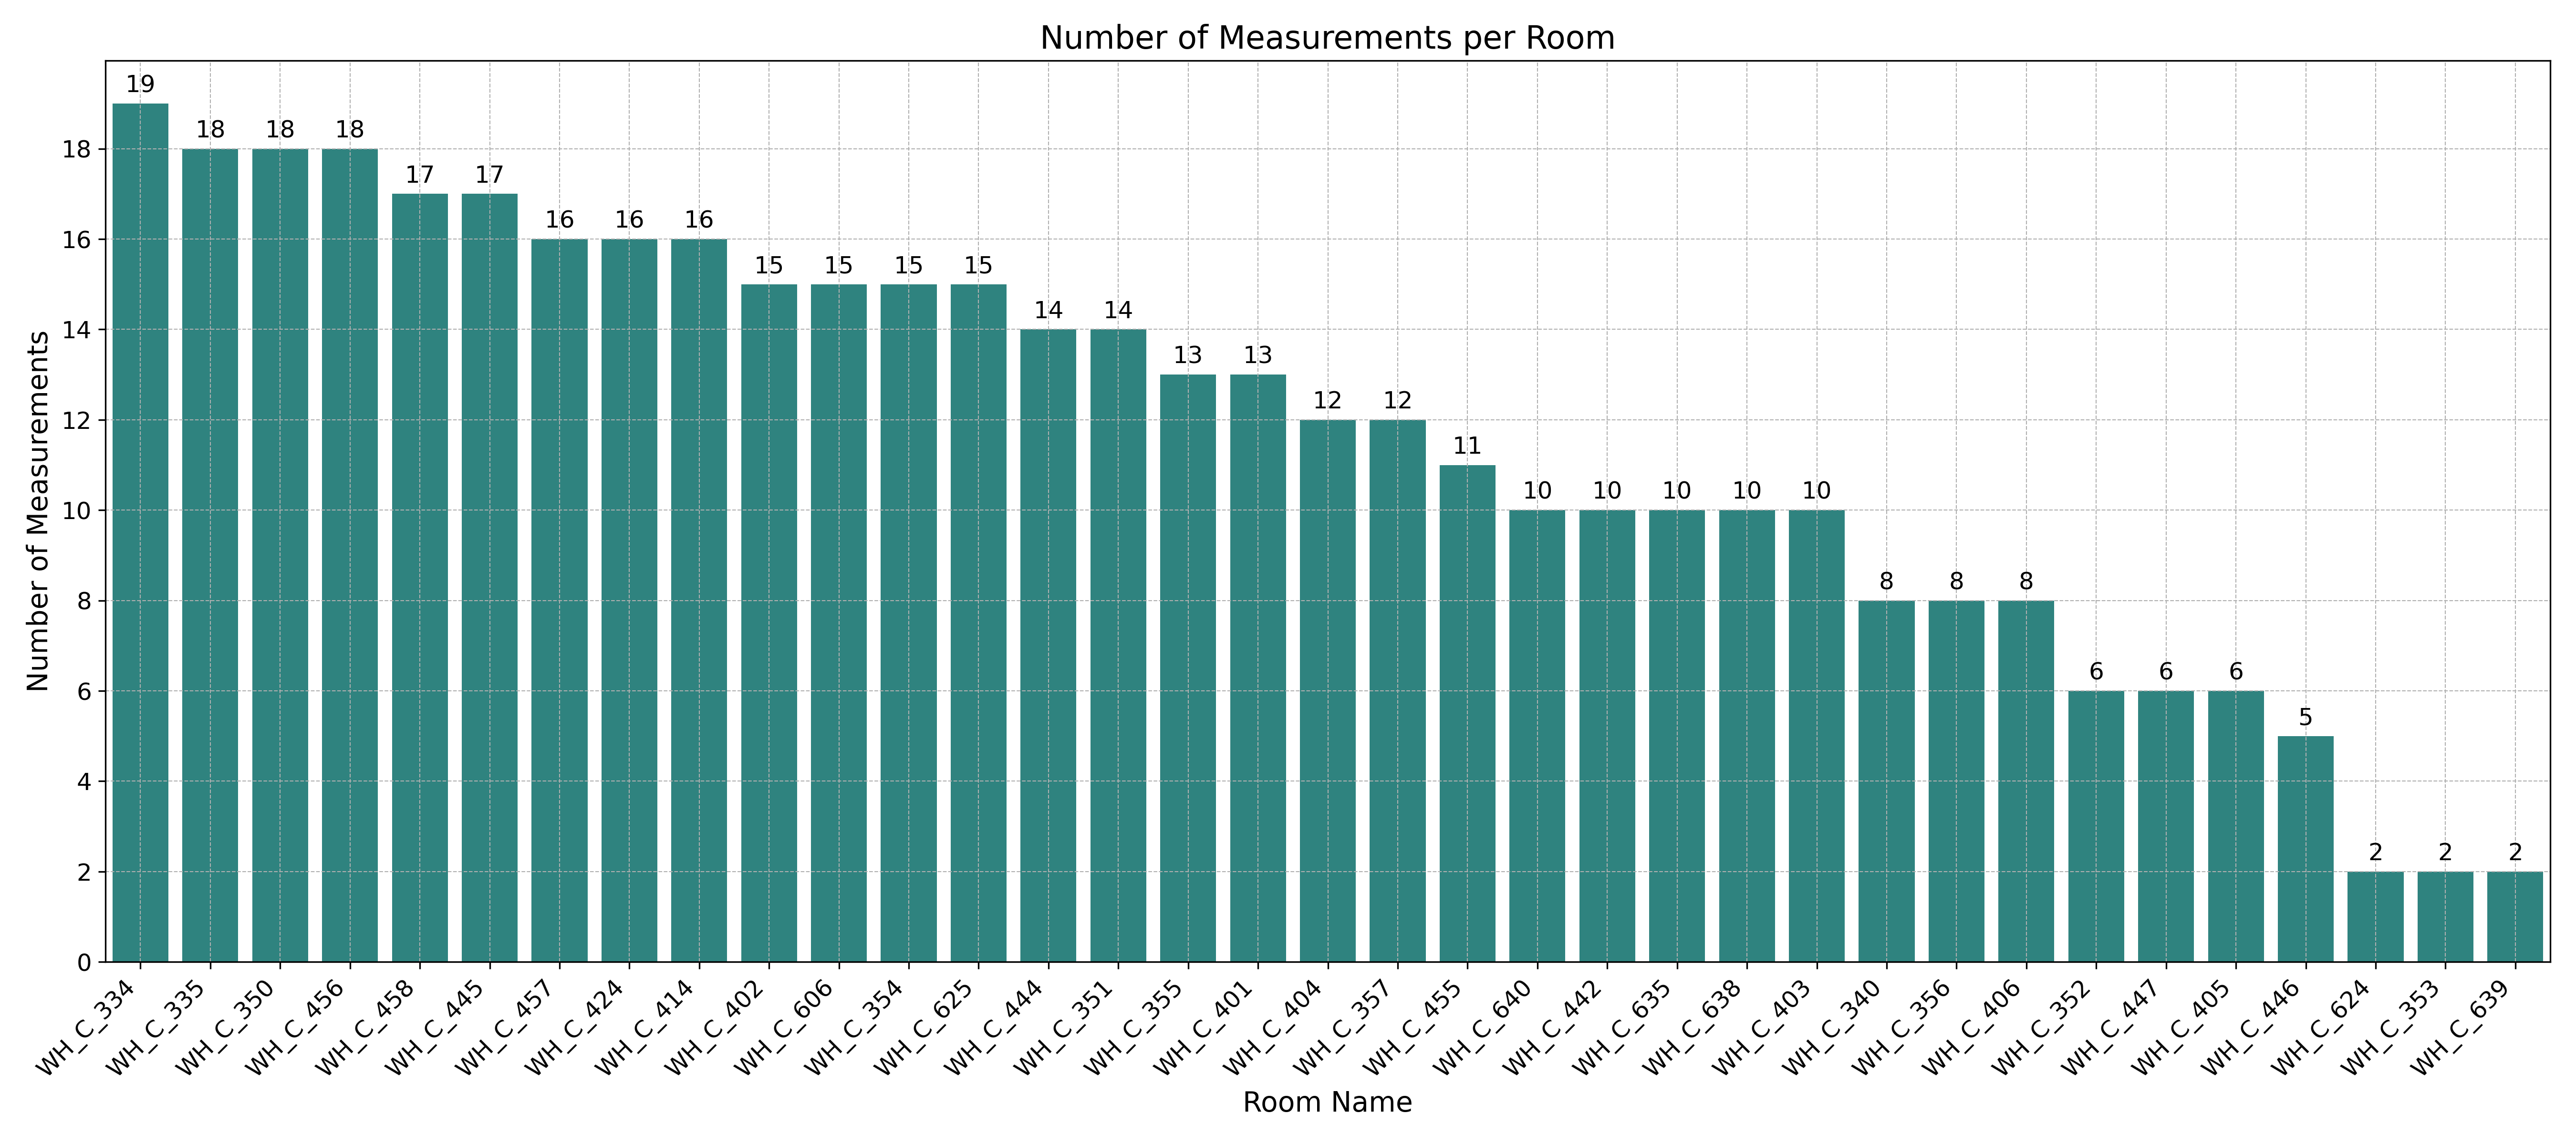
\includegraphics[width=0.8\textwidth]{images/0_general_01.png}
    \caption{Beispielabbildung 1}
    \label{fig:0_general_01}
\end{figure}

\begin{itemize}
    \item Verwendete Geräte (Doogee Y8, Google Pixel 8, Samsung Galaxy A?!)
\end{itemize}

\subsection{Methodik zur Untersuchung der Algorithmen}
\subsection{Detaillierte Beschreibung des Testprogramms}

\begin{itemize}
    \item \textbf{Programmübersicht:} Das Testprogramm dient dazu, die Leistungsfähigkeit verschiedener Machine Learning Algorithmen zur Indoor-Ortung basierend auf WiFi-Fingerprints zu evaluieren. Es lädt Konfigurationsparameter aus einer YAML-Datei, ruft Daten von einer API ab, filtert diese nach bestimmten Kriterien und vergleicht die Vorhersagen der Algorithmen unter verschiedenen Parametereinstellungen. Die Ergebnisse werden anschließend in CSV-Dateien gespeichert.

    \item \textbf{Ablauf und Logik:} Der Ablauf des Programms lässt sich wie folgt zusammenfassen:
          \begin{itemize}
              \item \textbf{Konfiguration laden:} Mit der Funktion \texttt{load\_config} wird die Konfigurationsdatei \texttt{config.yaml} geladen, die alle notwendigen Einstellungen und Parameter für die Tests enthält.
              \item \textbf{Erstellen des Ausgabeordners:} Die Funktion \texttt{create\_output\_directory} erstellt einen neuen Ordner, in dem die Ergebnisse gespeichert werden. Der Ordnername enthält einen Zeitstempel, um die Ergebnisse eindeutig zu identifizieren.
              \item \textbf{Daten abrufen:} Die Funktion \texttt{fetch\_data} ruft die WiFi-Fingerprint-Daten von einer angegebenen URL ab.
              \item \textbf{Daten filtern:} Falls in der Konfiguration Räume oder Korridore angegeben sind, werden die Daten mit der Funktion \texttt{filter\_data} entsprechend gefiltert.
              \item \textbf{Parameterkombinationen generieren:} Mit der Funktion \texttt{gene\allowbreak rate\_para\allowbreak meter\_\allowbreak com\allowbreak bi\allowbreak nations} werden alle möglichen Kombinationen der angegebenen Parameterwerte erstellt.
              \item \textbf{Vorhersagen und Vergleiche:} Die Funktion \texttt{compare\_predictions} vergleicht die Vorhersagen der Algorithmen mit den tatsächlichen Raumdaten. Die Ergebnisse werden in CSV-Dateien gespeichert, wobei jede Datei eine spezifische Parametereinstellung repräsentiert.
          \end{itemize}

    \item \textbf{Erweiterbarkeit und Anpassung:} Das Programm ist so aufgebaut, dass es leicht erweitert und angepasst werden kann. Neue Parameter oder Algorithmen können einfach in die YAML-Konfigurationsdatei hinzugefügt werden. Die modularen Funktionen ermöglichen es, einzelne Teile des Programms bei Bedarf zu modifizieren oder zu ersetzen, ohne die gesamte Codebasis ändern zu müssen.
\end{itemize}

\subsubsection{Konfiguration über YAML-Dateien}
\begin{itemize}
    \item \textbf{Konfigurationsdateien:} Die Konfiguration des Programms erfolgt über eine YAML-Datei (\texttt{config.yaml}), die alle notwendigen Parameter und Einstellungen enthält. Diese Datei ermöglicht eine flexible Anpassung des Testprozesses, ohne dass der Quellcode selbst verändert werden muss.

    \item \textbf{Parameter und Einstellungen:} Die YAML-Datei enthält folgende Hauptparameter:
          \begin{itemize}
              \item \textbf{url\_fetch:} Die URL, von der die WiFi-Fingerprint-Daten abgerufen werden.
              \item \textbf{url\_predict:} Die URL der API, die für die Vorhersagen verwendet wird.
              \item \textbf{num\_measurements:} Die Anzahl der Messungen, die verarbeitet werden sollen.
              \item \textbf{rooms und corridors:} Listen von Raum- und Korridornamen, die in die Analyse einbezogen werden sollen.
              \item \textbf{parameter\_sets:} Verschiedene Sätze von Parametern, die für die Vorhersagen verwendet werden. Jeder Satz enthält spezifische Werte für Algorithmen und deren Einstellungen.
          \end{itemize}

    \item \textbf{Anwendungsbeispiele:} Ein typisches Beispiel für die YAML-Konfigurationsdatei sieht wie folgt aus:
          \begin{lstlisting}[caption=.yaml Konfigurationsdatei, label={lst:code_yaml}]
url_fetch: "http://127.0.0.1:5000/measurements/all"
url_predict: "http://127.0.0.1:5000/measurements/predict"
num_measurements: 10
rooms: ["WH_C_334", "WH_C_335"]
corridors: ["WH_C_352"]
parameter_sets:
    - name: "test"
    parameters:
        router_selection: ['all']
        handle_missing_values_strategy: ['-100']
        router_presence_threshold: [0]
        router_rssi_threshold: [-100]
        value_scaling_strategy: ['none']
        weights: ["distance"]
        algorithm:
            knn_euclidean:
                k_value: [7]
        \end{lstlisting}
          Diese Konfiguration spezifiziert, dass die Daten von \texttt{http://127.0.0.1:5000/\discretionary{}{}{}measure\discretionary{}{}{}ments/\discretionary{}{}{}all} abgerufen und die Vorhersagen bei \texttt{http://127.0.0.1:5000/\discretionary{}{}{}measure\discretionary{}{}{}ments/\discretionary{}{}{}predict} gemacht werden sollen. Es sollen 10 Messungen verarbeitet werden, die entweder in den angegebenen Räumen oder Korridoren aufgenommen wurden. Der Parameter \texttt{parameter\_sets} definiert verschiedene Sätze von Parametern, die für die Vorhersagen verwendet werden.
\end{itemize}



\section{Vergleich der Algorithmen und Parameter}
\subsection{Untersuchung der Genauigkeit in Abhängigkeit von Parametern}

1. Auswahl der nicht konkret betrachteten Parameter bei KNN und SVM

KNN (weights: distance vs. uniform):

\begin{figure}[H]
    \centering
    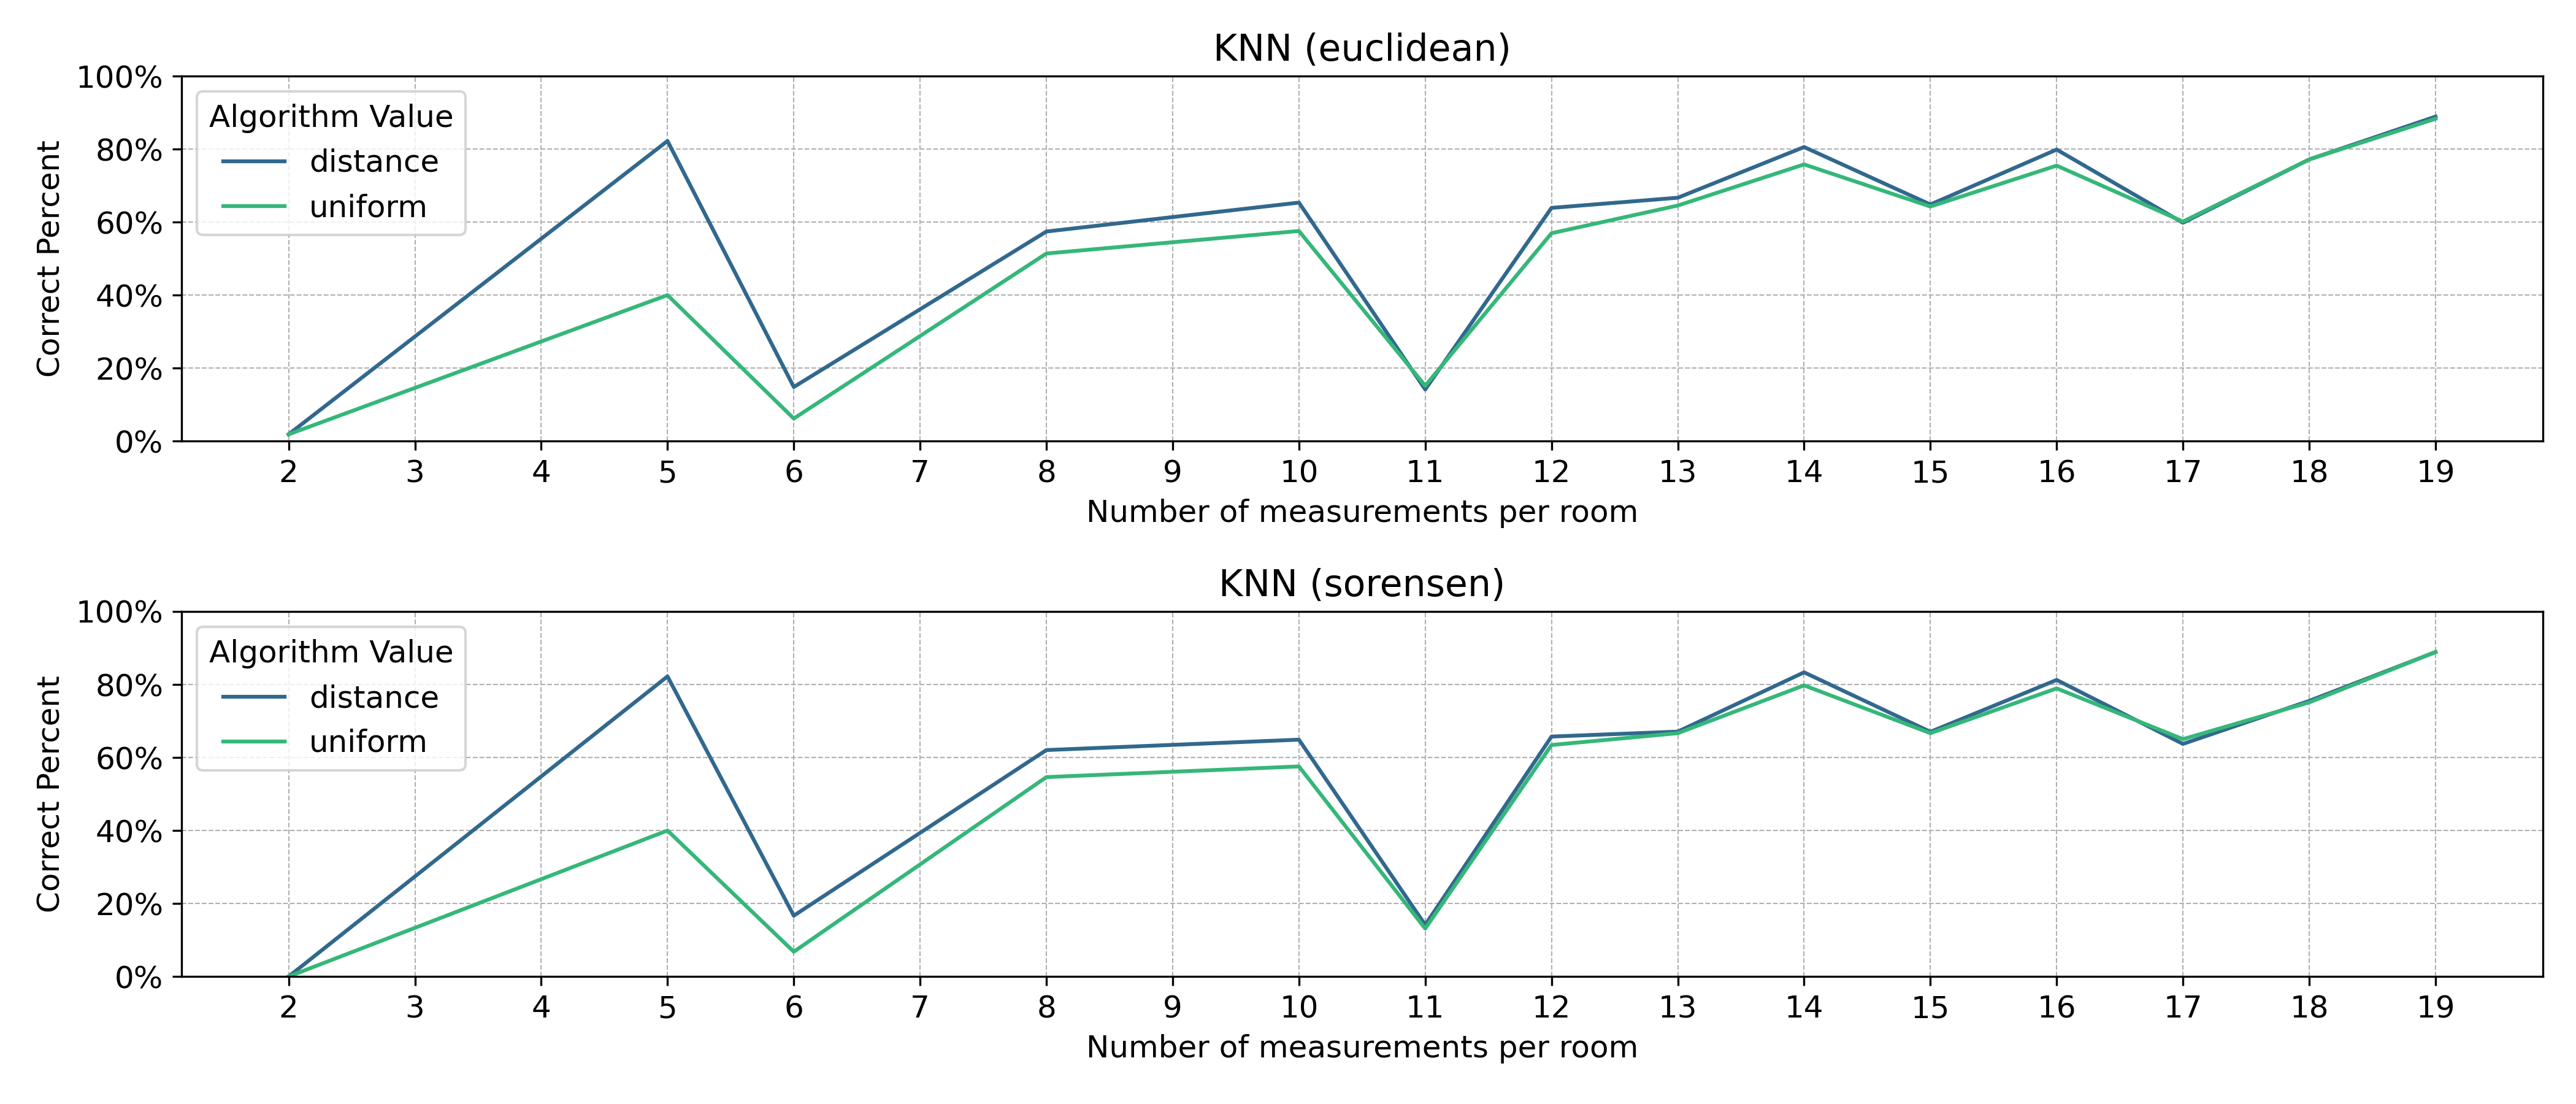
\includegraphics[width=0.8\textwidth]{images/1_distance_uniform_weights_01.png}
    \caption{Distance vs. Uniform weights}
    \label{fig:1_distance_uniform_weights_01}
\end{figure}

Ergebnis: Distance ist besser als Uniform

SVM (RBF) (gamma: scale vs. auto):

\begin{figure}[H]
    \centering
    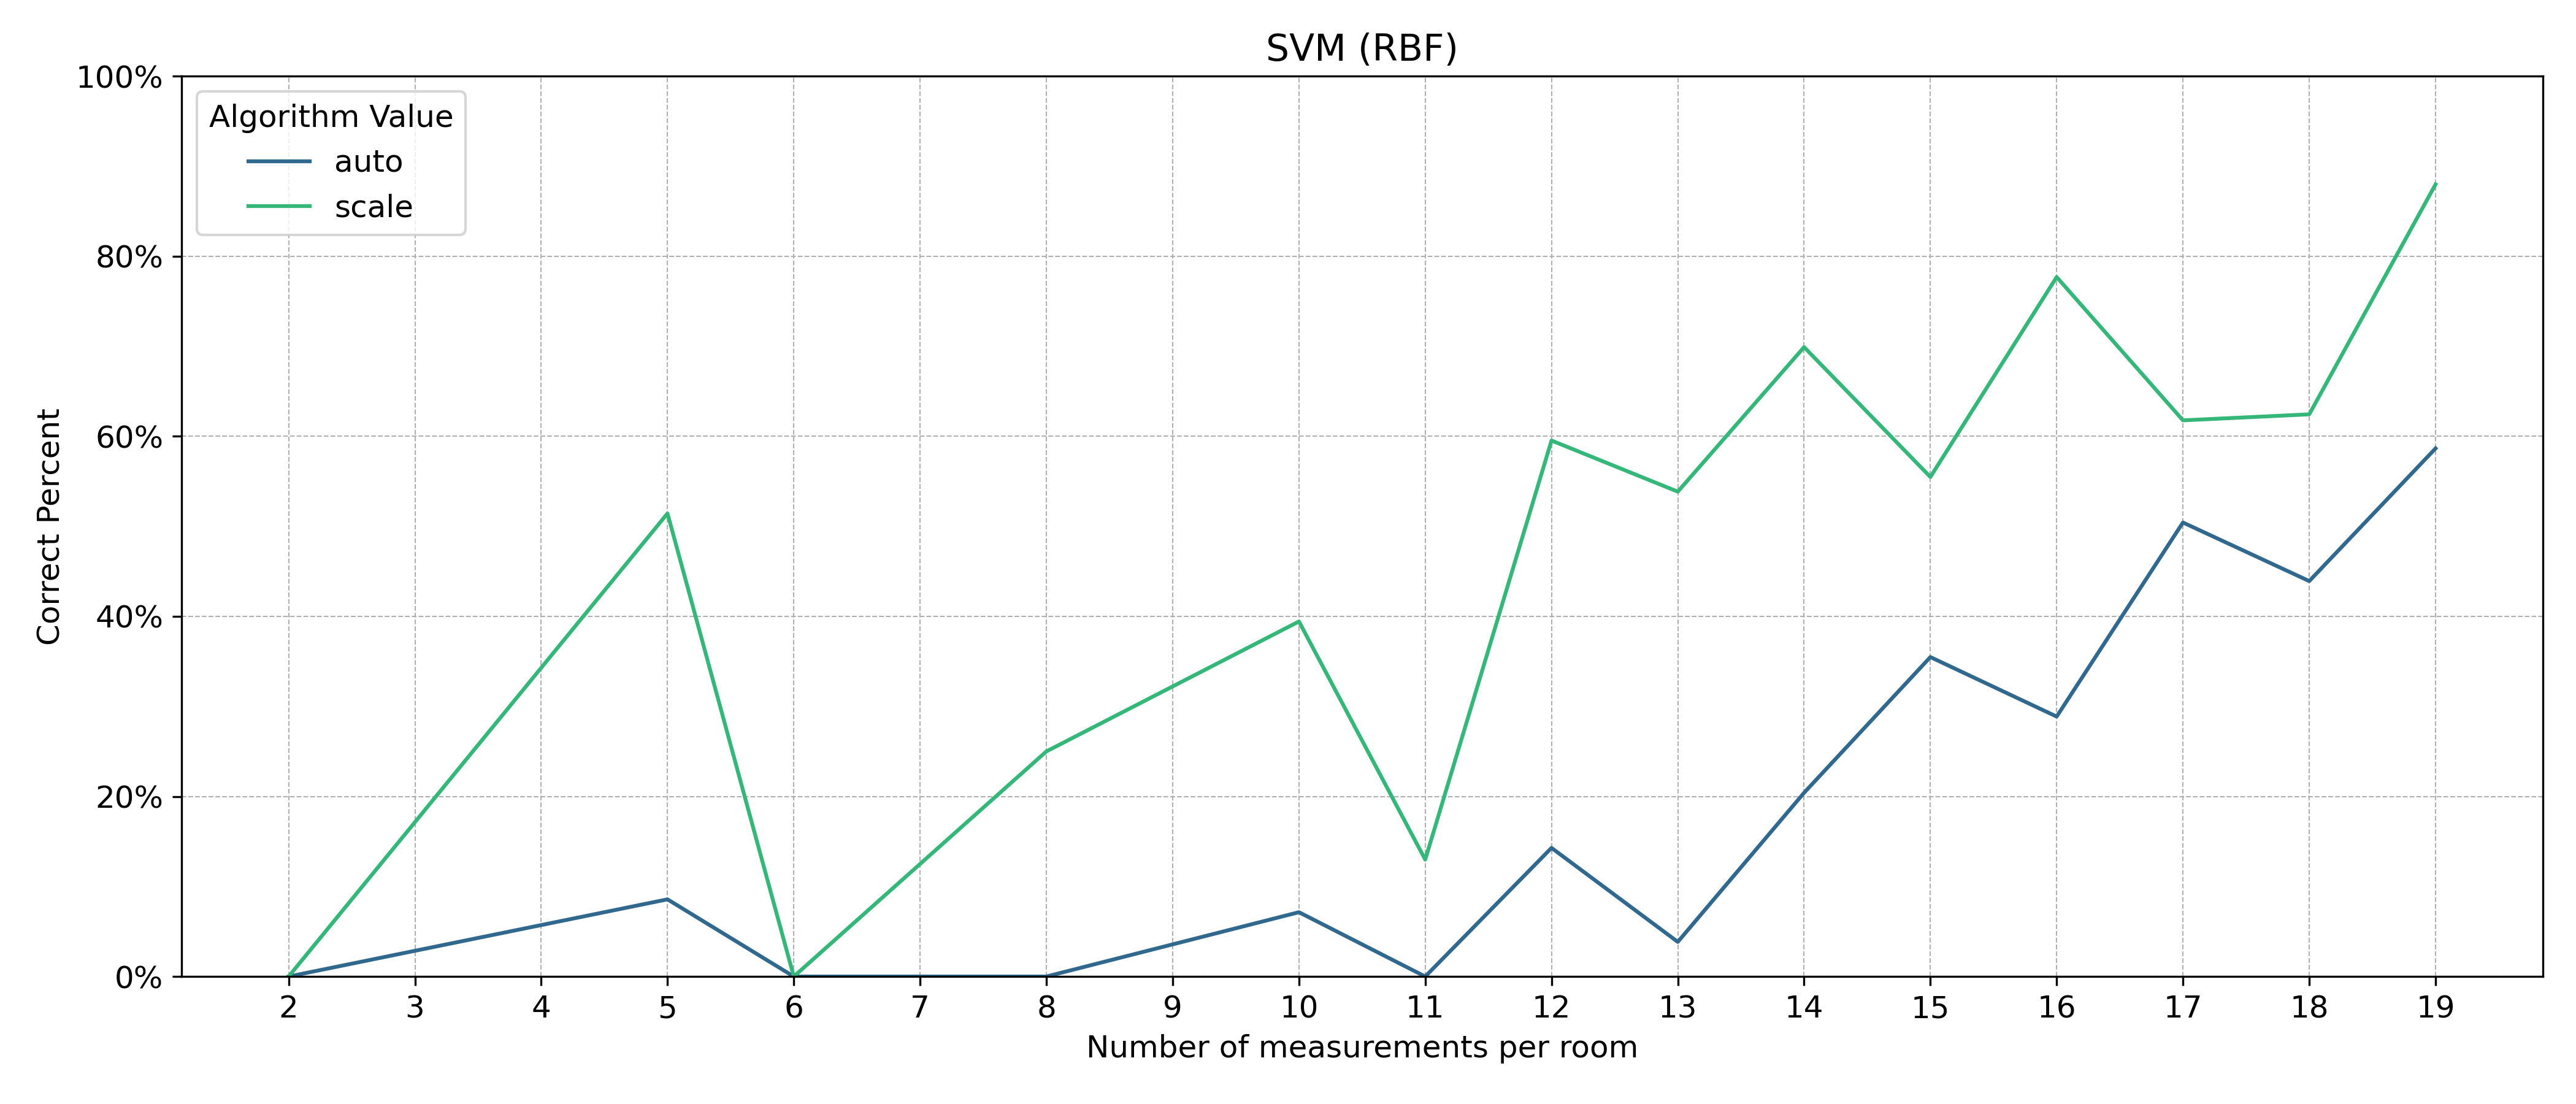
\includegraphics[width=0.8\textwidth]{images/1_best_parameters_svm_01.png}
    \caption{Scale vs. Auto bei SVM RBF}
    \label{fig:1_best_parameters_svm_01}
\end{figure}

Ergebnis: Scale ist besser als Auto

TODO: In welchem Wertebereich liegen die Werte?

TODO:
\begin{itemize}
    \item Es muss auch irgendwo stehen was der average und der weighted average ist und warum beides in den Plots gezeigt wird!
\end{itemize}

In Abbildung \ref{fig:2_best_parameters_01} sind die besten Parameter für die Algorithmen in Abhängigkeit der Anzahl der Messungen dargestellt. Die Parameter wurden durch die Anwendung des Testprogramms auf die gesammelten Daten ermittelt. Die Parameter wurden so gewählt, dass die Genauigkeit der Algorithmen maximiert wurde. In Abbildung \ref{fig:2_best_parameters_02} ist die durchschnittliche Genauigkeit der Parameter dargestellt. Die Genauigkeit wurde durch die Anwendung des Testprogramms auf die gesammelten Daten ermittelt.

\begin{figure}[H]
    \centering
    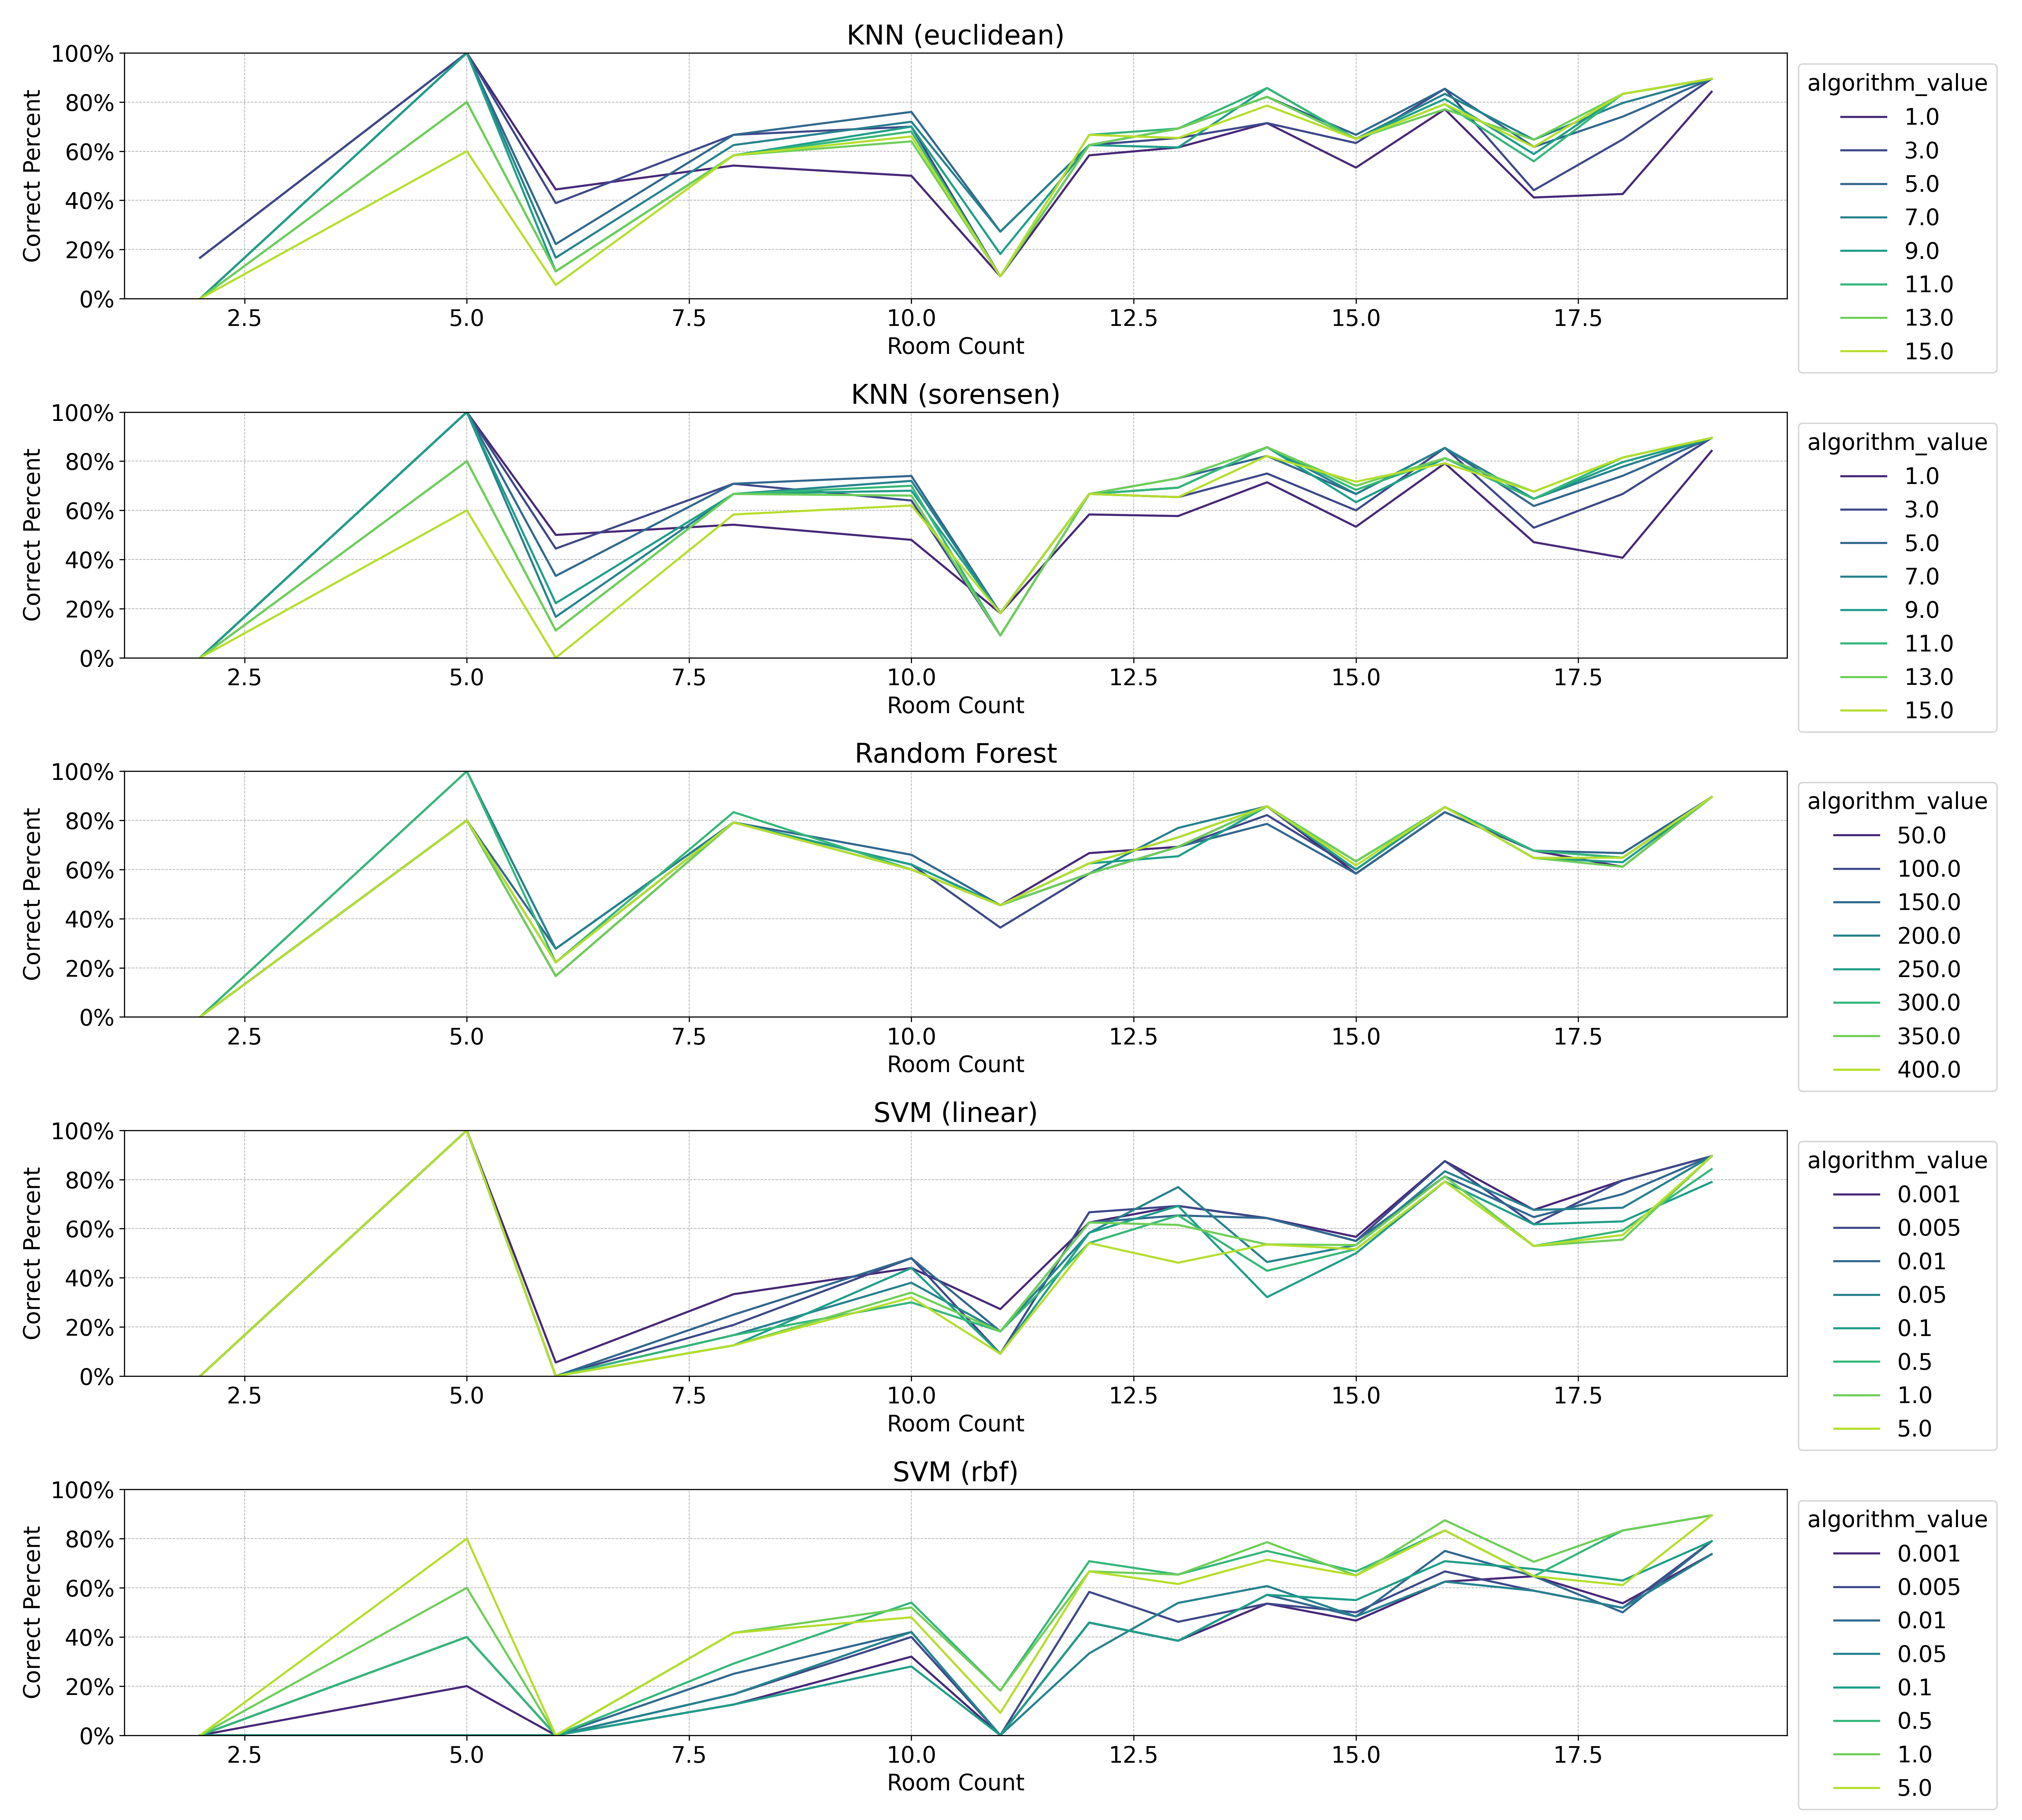
\includegraphics[width=0.8\textwidth]{images/2_best_parameters_01.png}
    \caption{Vergleich der Parameter in Abhängigkeit der Anzahl der Messungen}
    \label{fig:2_best_parameters_01}
\end{figure}

\begin{figure}[H]
    \centering
    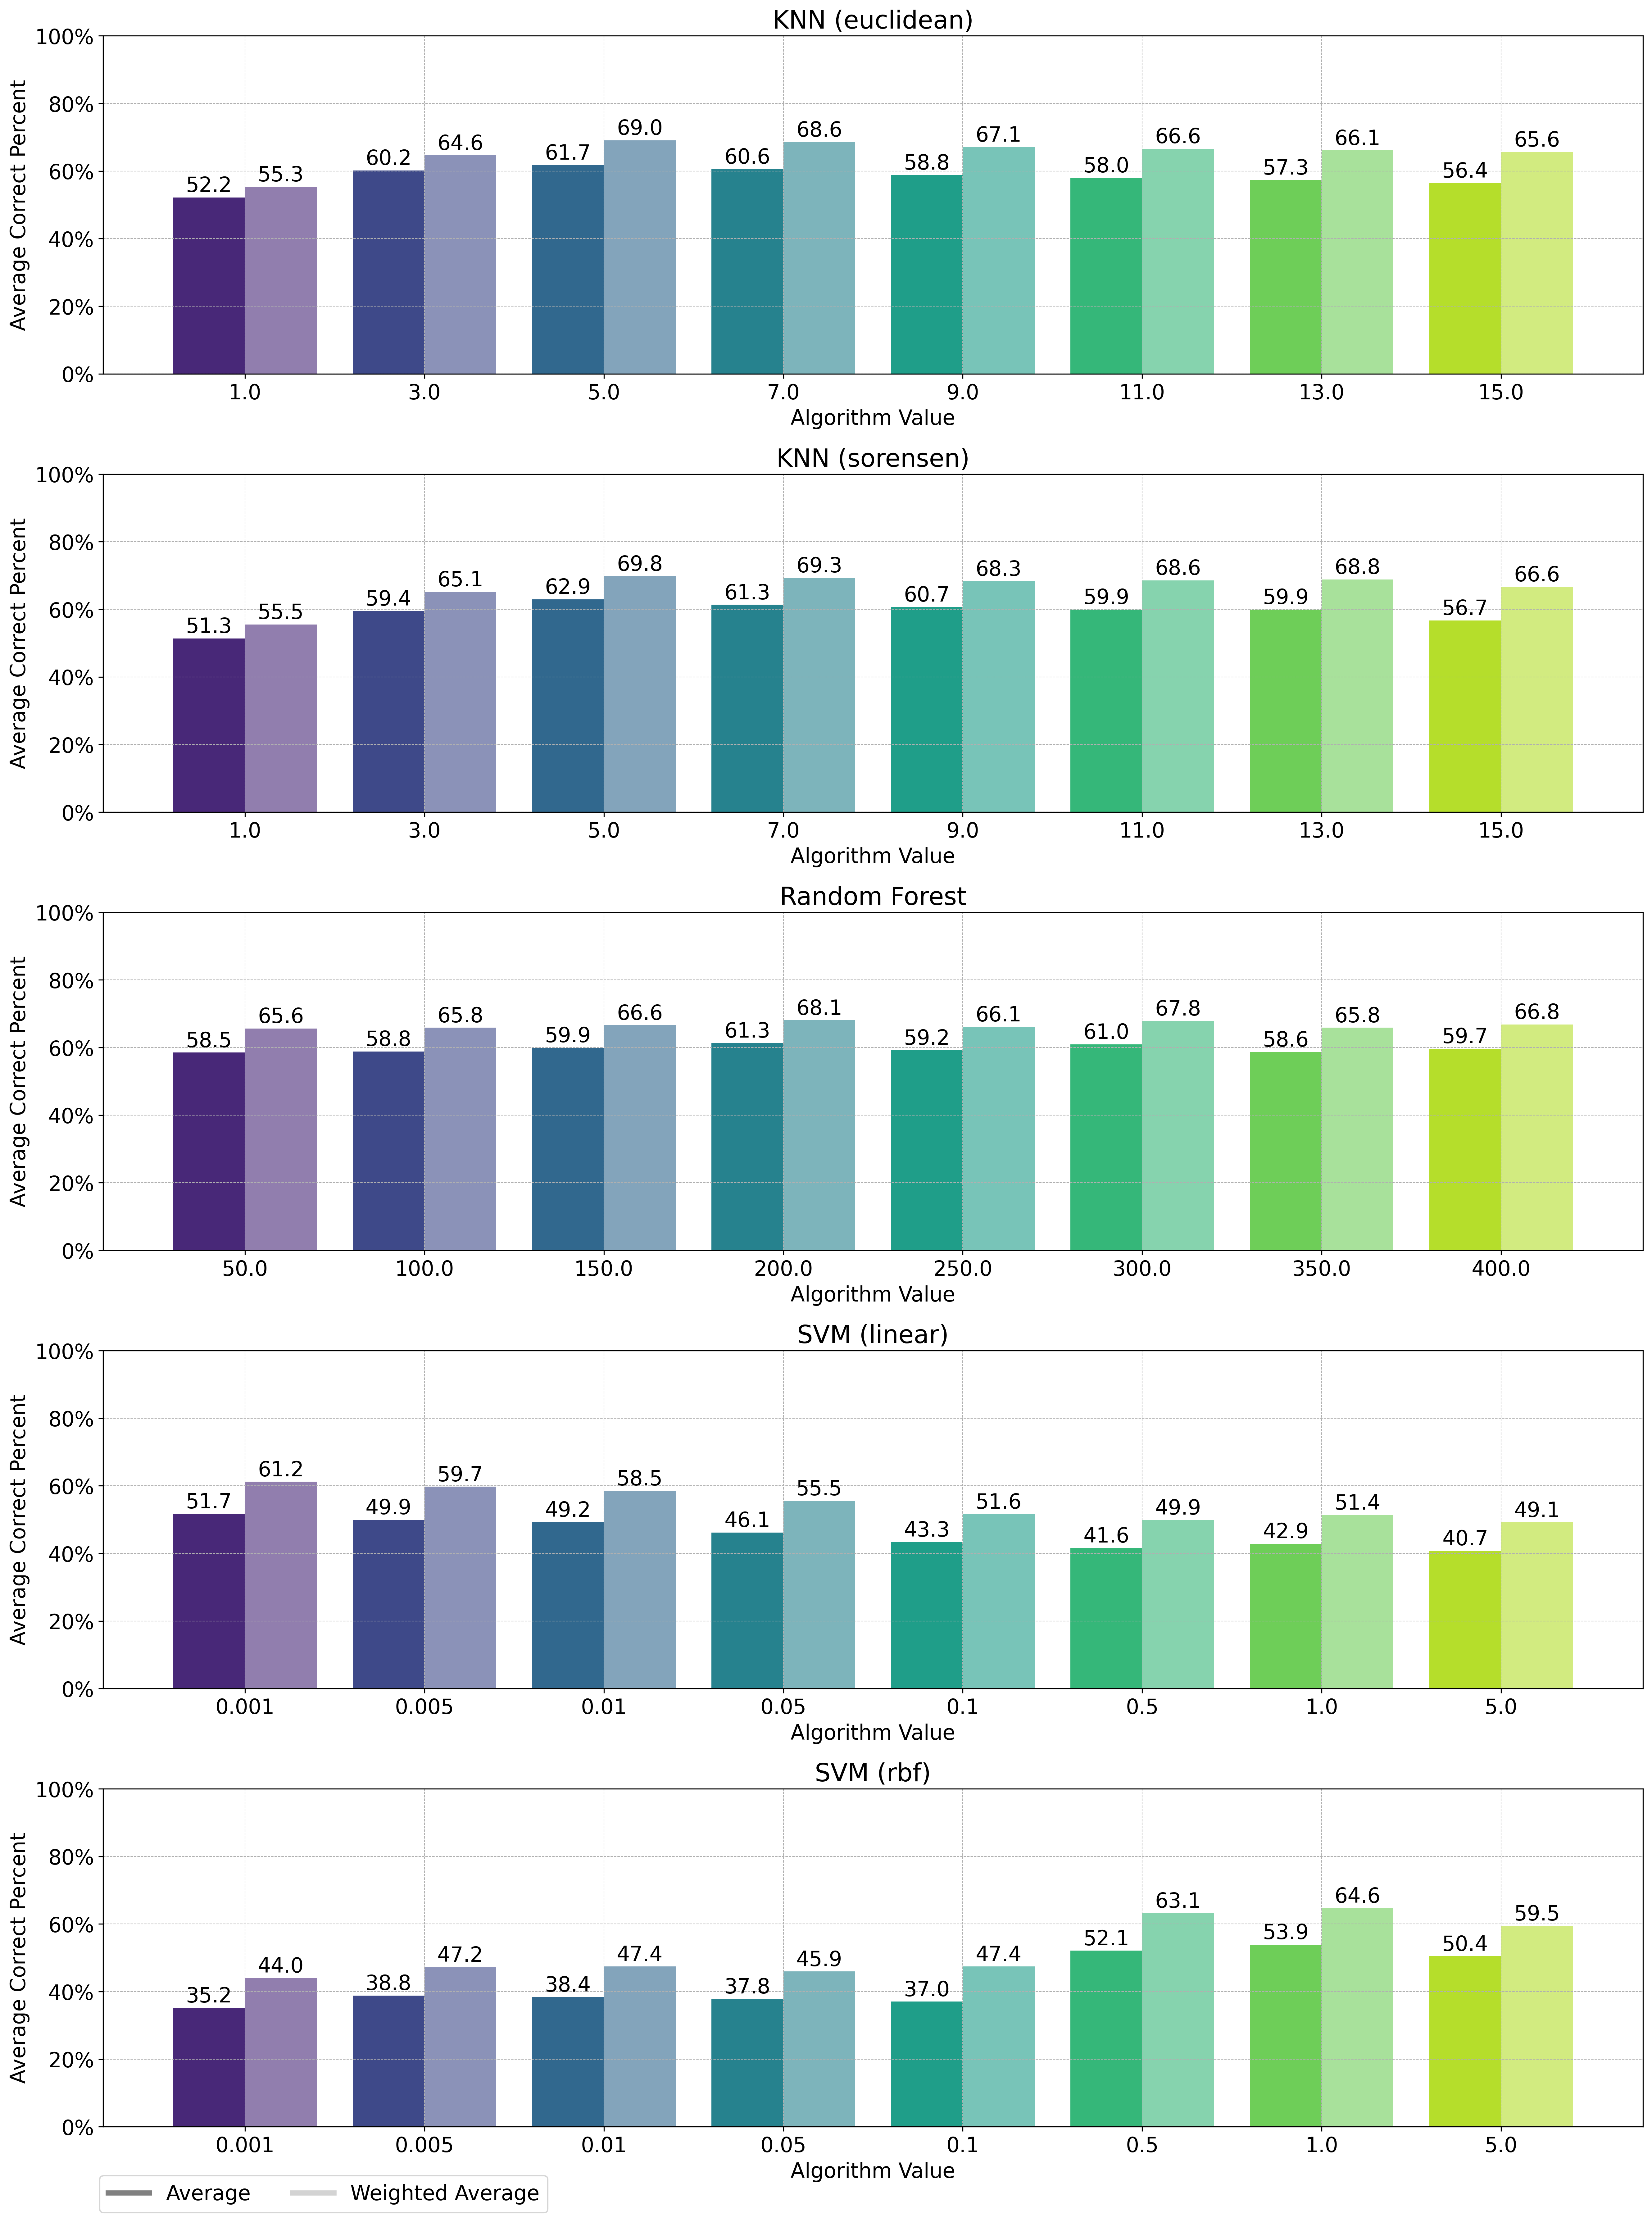
\includegraphics[width=0.8\textwidth]{images/2_best_parameters_02.png}
    \caption{Vergleich der durschnittlichen Genauigkeit der Parameter}
    \label{fig:2_best_parameters_02}
\end{figure}

Warum diese Parameter?
\begin{itemize}
    \item KNN: 1, 3, 5, 7, 9, 11, 13, 15 -> Weil ungerade (siehe Quelle bei KNN), im Wertebereich der Anzahl an Messungen pro Raum
    \item RF: 50, 100, 150, 200, 250, 300, 350, 400 Wurde gewählt, weil 407 Messpunkte existieren
    \item SVM: 0.001, 0.005, 0.01, 0.05, 0.1, 0.5, 1, 5 -> Quelle: Supervised Learning-Based Indoor Positioning System Using WiFi Fingerprints Seite 62
\end{itemize}

Ergebnisse:

\begin{itemize}
    \item KNN: 5, 7, 9
    \item RF: 100, 200, 300
    \item SVM (RBF): 0.5, 1, 5
    \item SVM (Linear): 0.001, 0.005, 0.01
\end{itemize}

\paragraph{KNN}
% \linebreak

Bei der KNN-Analyse wurden die Werte 5, 7 und 9 für k ausgewählt. Wie in Abbildung \ref{fig:2_best_parameters_01} zu sehen ist, zeigen die Genauigkeiten, dass bei Räumen mit wenigen Messungen kleinere k-Werte bessere Ergebnisse liefern, während bei Räumen mit mehr Messungen größere k-Werte vorteilhafter sind. Diese Tendenz ist sowohl bei der euclidean- als auch bei der sorensen-Metrik zu beobachten.


Abbildung \ref{fig:2_best_parameters_02} zeigt, dass bei average/euclidean die Werte 3, 5 und 7 die besten Ergebnisse liefern, während bei weighted average/euclidean die Werte 5, 7 und 9 am besten abschneiden. Bei average/sorensen erzielen die Werte 5, 7 und 9 die besten Ergebnisse, und bei weighted average/sorensen sind es die Werte 5, 7 und 13, wobei die Genauigkeit bei k = 9 und k = 11 kaum von der Genauigkeit bei k = 13 abweicht.

Generell ist die Genauigkeit bei mehreren Messungen pro Raum weniger stark von k abhängig als bei wenigen Messungen pro Raum, mit Ausnahme von sehr kleinen k-Werten wie 1 oder 3. Daher wurden für die weiteren Analysen die k-Werte 5, 7 und 9 gewählt.

\paragraph{Random Forest}
% \linebreak

Wie in Abbildung \ref{fig:2_best_parameters_01} zu sehen ist, hat der Wert für n\_estimators beim Random-Forest-Algorithmus keinen großen Einfluss. Aus diesem Grund wurden die Werte 100, 300 und 500 gewählt, um eine gleichmäßige Verteilung zu gewährleisten.

\paragraph{SVM (linear)}
% \linebreak


Interessanterweise wurden bei der linearen SVM unabhängig vom Parameter C alle Räume korrekt vorhergesagt. Sollte man vielleicht in Betracht ziehen, alle Räume mit nur 5 Messungen zu verwenden und den SVM-Algorithmus anzuwenden? Die Ursache könnte Zufall sein (weniger Messungen führen zu größerer Streuung) oder der Algorithmus ist tatsächlich so gut. Ansonsten nimmt die Genauigkeit mit zunehmendem Wert für C ab. Die besten Werte bei average und weighted average wurden für die Werte 0,001, 0,005 und 0,01 erzielt. Daher wurden für die weitere Analyse die Werte C = 0.001, 0.005 und 0.01 gewählt.

\paragraph{SVM (rbf)}
% \linebreak

Generell lässt sich in Abbildung \ref{fig:2_best_parameters_01} erkennen, dass größere Werte für C bessere Ergebnisse liefern als kleinere. Die besten Ergebnisse konnten bei average und weighted average für C = 1.0 erzielt werden. Daher wurden für die weitere Analyse die Werte C = 0.5, 1.0 und 5.0 gewählt.

\subsection{Strategien zum Umgang mit fehlenden Werten}

In Abbildung \ref{fig:3_handle_missing_values_strategy_01} ist die Genauigkeit der Algorithmen in Abhängigkeit der Strategie zum Umgang mit fehlenden Werten dargestellt. Die Strategien wurden durch die Anwendung des Testprogramms auf die gesammelten Daten ermittelt. Die Genauigkeit wurde durch die Anwendung des Testprogramms auf die gesammelten Daten ermittelt.

\begin{figure}[H]
    \centering
    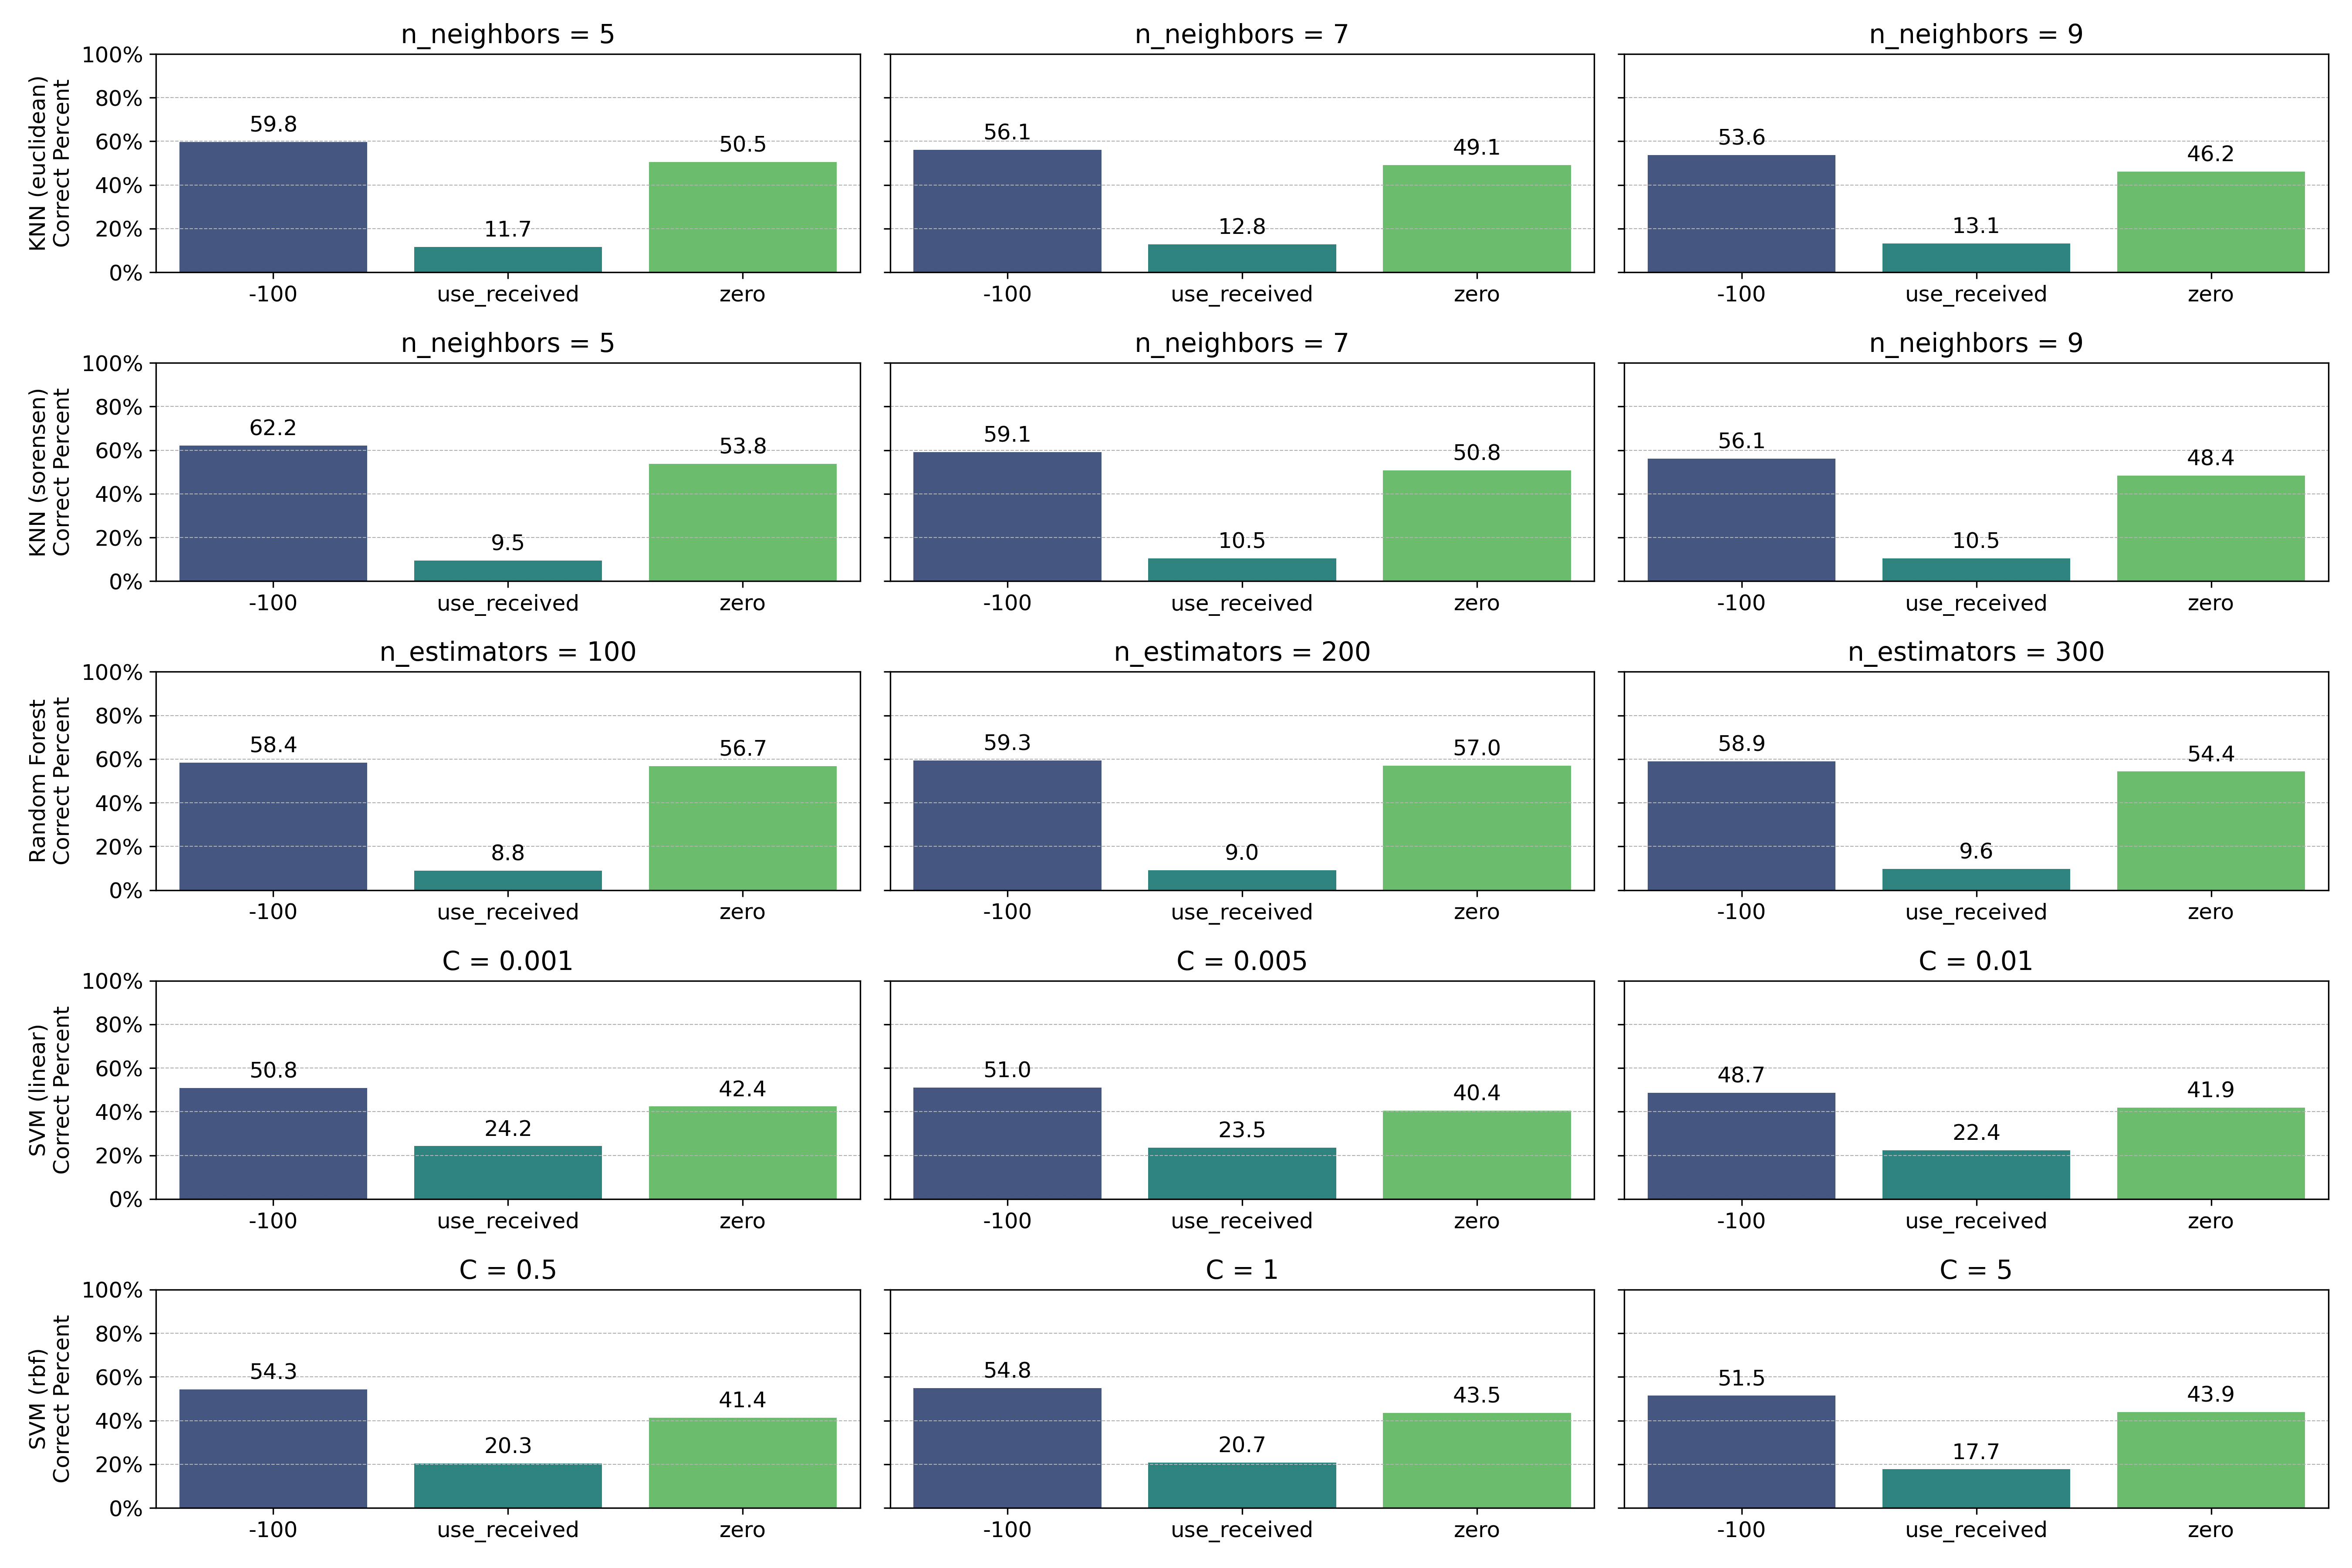
\includegraphics[width=0.8\textwidth]{images/3_handle_missing_values_strategy_01.png}
    \caption{Vergleich der Genauigkeit in Abhängigkeit der Strategie zum Umgang mit fehlenden Werten}
    \label{fig:3_handle_missing_values_strategy_01}
\end{figure}

\subsection{Einfluss der verwendeten Router}

Die Ergebnisse der verschiedenen Strategien zur Auswahl der Router sind in Abbildung \ref{fig:4_router_selection_02} dargestellt.

\begin{itemize}
    \item Alle Router sind besser als nur die eduroam Router
    \item Unterschiede nehmen mit zunehmener Anzaahl der Messungen eines Raums ab.
    \item Es wird sich trotzdem für alle Router entschieden, da die Unterschiede hauptsächlich bei wenigen Messungen auftreten und dort eine größere Streuung erwaret wird und bei den eduroam Routern sichergestellt werden kann, dass diese nicht die Position verändern
\end{itemize}

\begin{figure}[H]
    \centering
    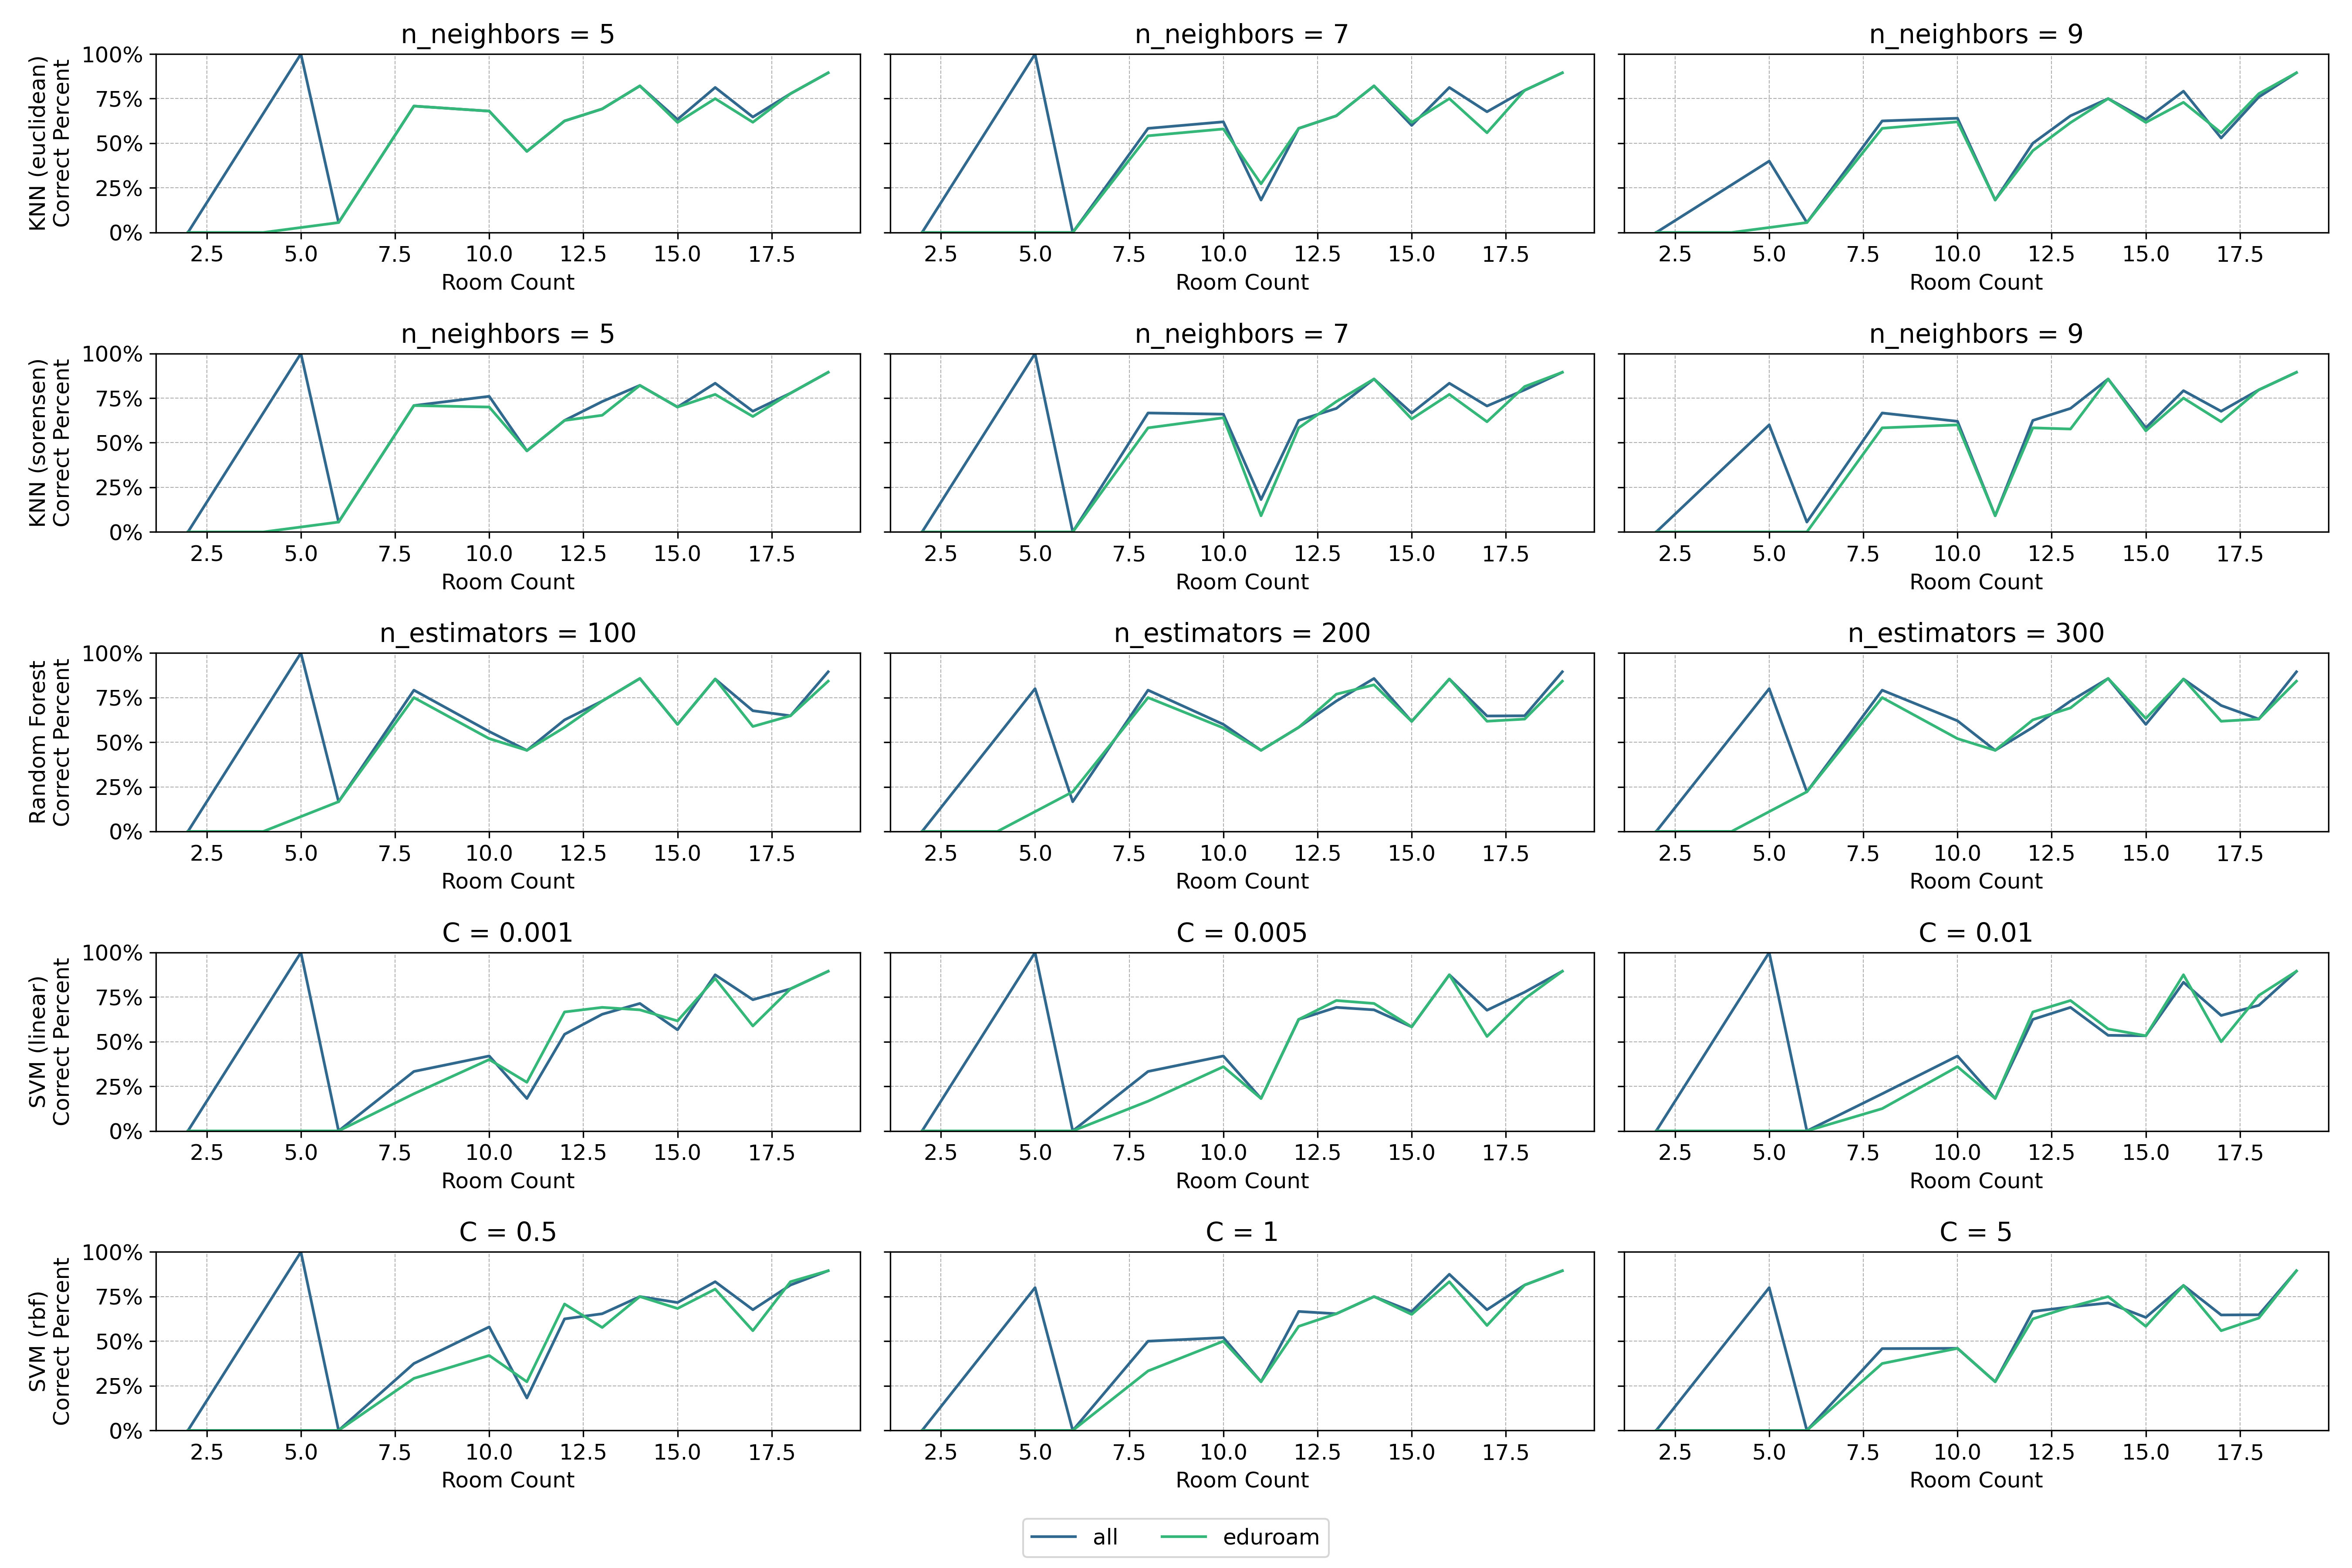
\includegraphics[width=0.8\textwidth]{images/4_router_selection_02.png}
    \caption{Auswahl der Router}
    \label{fig:4_router_selection_02}
\end{figure}

\subsection{Filterung von RSSI-Werten}
\subsubsection{Berücksichtigung nur häufig auftretender Router}

Die Ergebnisse der verschiedenen Strategien zur Auswahl des Router Presence Threshold sind in Abbildung \ref{fig:5_router_presence_threshold_02} dargestellt.

\begin{itemize}
    \item Router die in mehreren Messungen eines Raums vorhanden sind, sind aussagekräftiger als Router die nur in wenigen Messungen vorhanden sind
    \item Also: In wie viel Prozent der Messungen muss ein Router vorhanden sein, damit er berücksichtigt wird
    \item Das bedeutet, dass bei wenig Messungen die Auswirkungen gering sein sollten
\end{itemize}

\begin{itemize}
    \item bei allen Algorithmen ist 0 am besten
    \item Interessant: Bei allen Algos haben die Genauigkeiten in Abhängigkkeit der Messungen pro Raum einen ähnlichen Verlauf und sind mit zunehmendem Router Presence Threshold schlechter, AUSSER bei SVM. Doer sind bei wenigen Messungen die größeren Router Presence Thresholds besser und bei mehr Messungen die kleineren. -> Deswegen wurde hier 0.25 verwendet, da dieser Wert im Schnitt die besten Ergebnisse erzielt
    \item SVM-Kipppunkt bei 10
\end{itemize}

\begin{figure}[H]
    \centering
    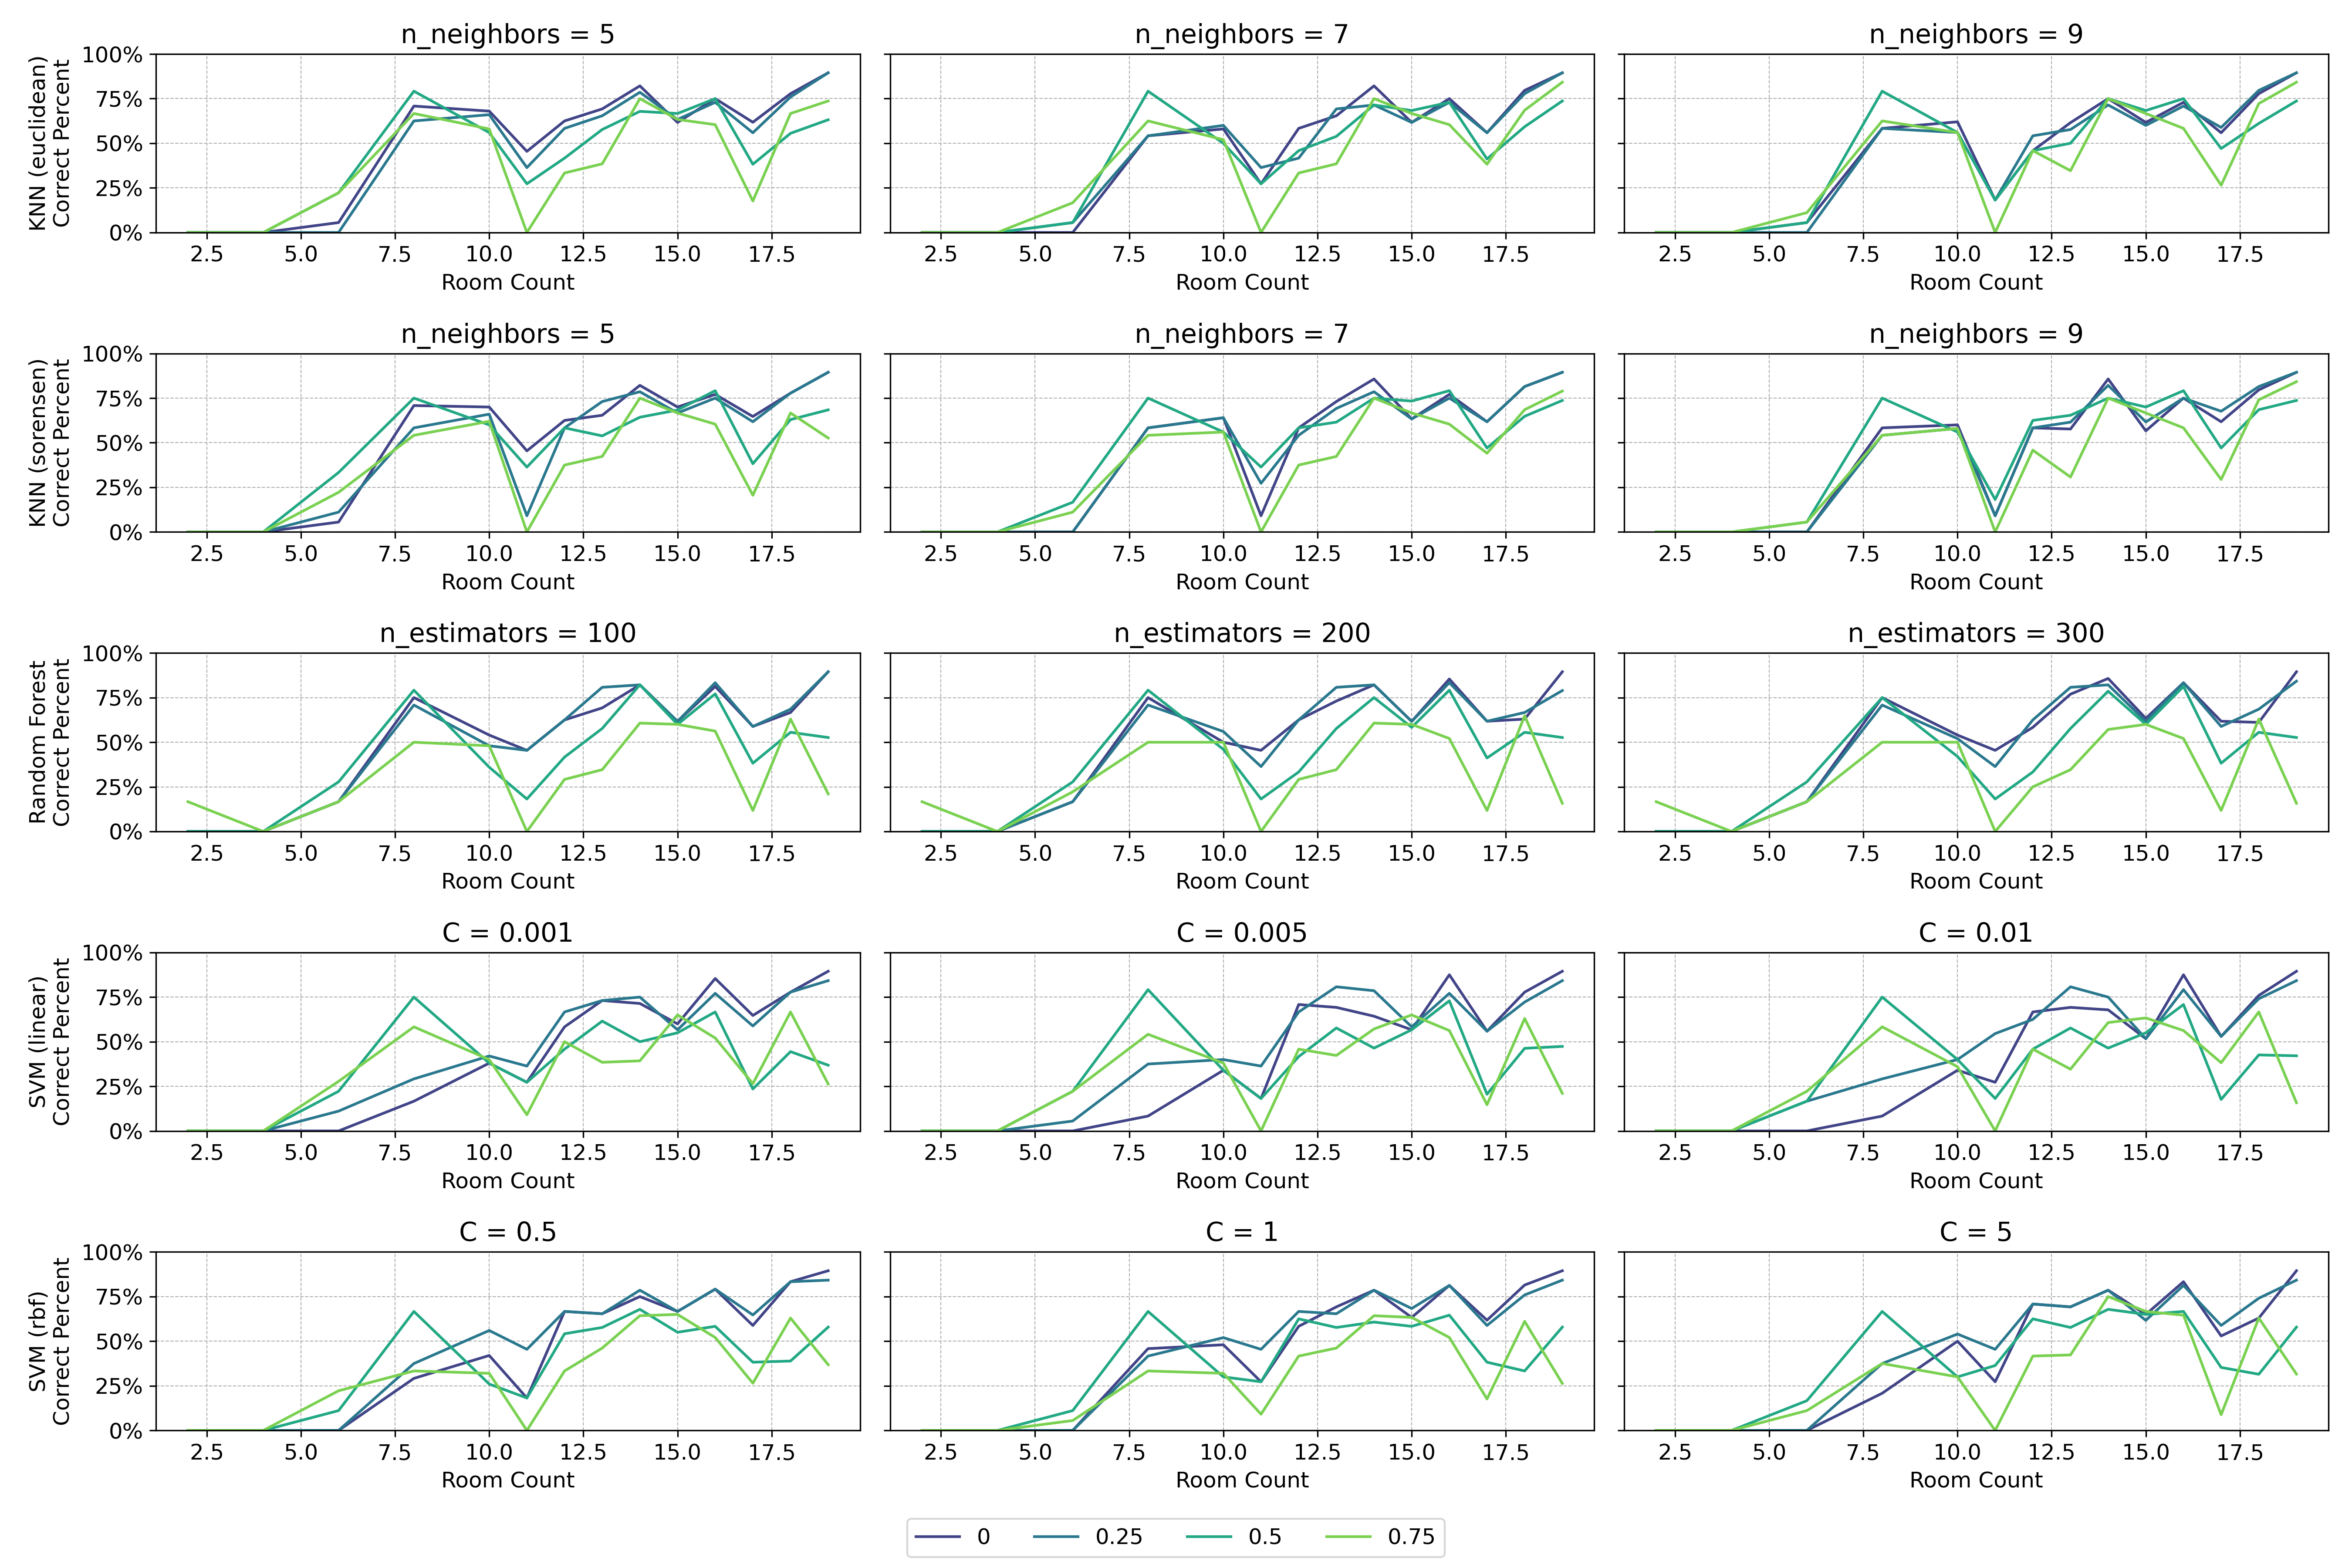
\includegraphics[width=0.8\textwidth]{images/5_router_presence_threshold_02.png}
    \caption{Vergleich der Genauigkeit in Abhängigkeit des Schwellenwerts für die Anzahl der Messungen eines Routers}
    \label{fig:5_router_presence_threshold_02}
\end{figure}

\subsubsection{Ausschluss von Routern mit schwachem Signal}

Die Ergebnisse der verschiedenen Strategien zur Auswahl des Router Rssi Threshold sind in Abbildung \ref{fig:6_router_rssi_threshold_01} dargestellt.

\begin{itemize}
    \item Idee: sehr kleine RSSI Werte werden ignoriert/so getan, als wäre die bei der Messung nicht dabei
    \item Gedanke dahiner: Router mit größeren RSSI-Werten sind aussagekräftiger und sollten dadurch mehr Einfluss haben
    \item Ergebnis: Bei allen Algorithmen ist -100 am besten -> Router mit geringen RSSI-Werten haben einen größeren Einfluss als vermutet
    \item Idee ist nicht von mir, sondern kommt aus dem Paper: Quelle: Comprehensive analysis of distance and similarity measures for Wi-Fi fingerprinting indoor positioning systems
    \item Die Thresholds sind: -100, -90, -80, -70, -60, -50, -40
\end{itemize}

\begin{figure}[H]
    \centering
    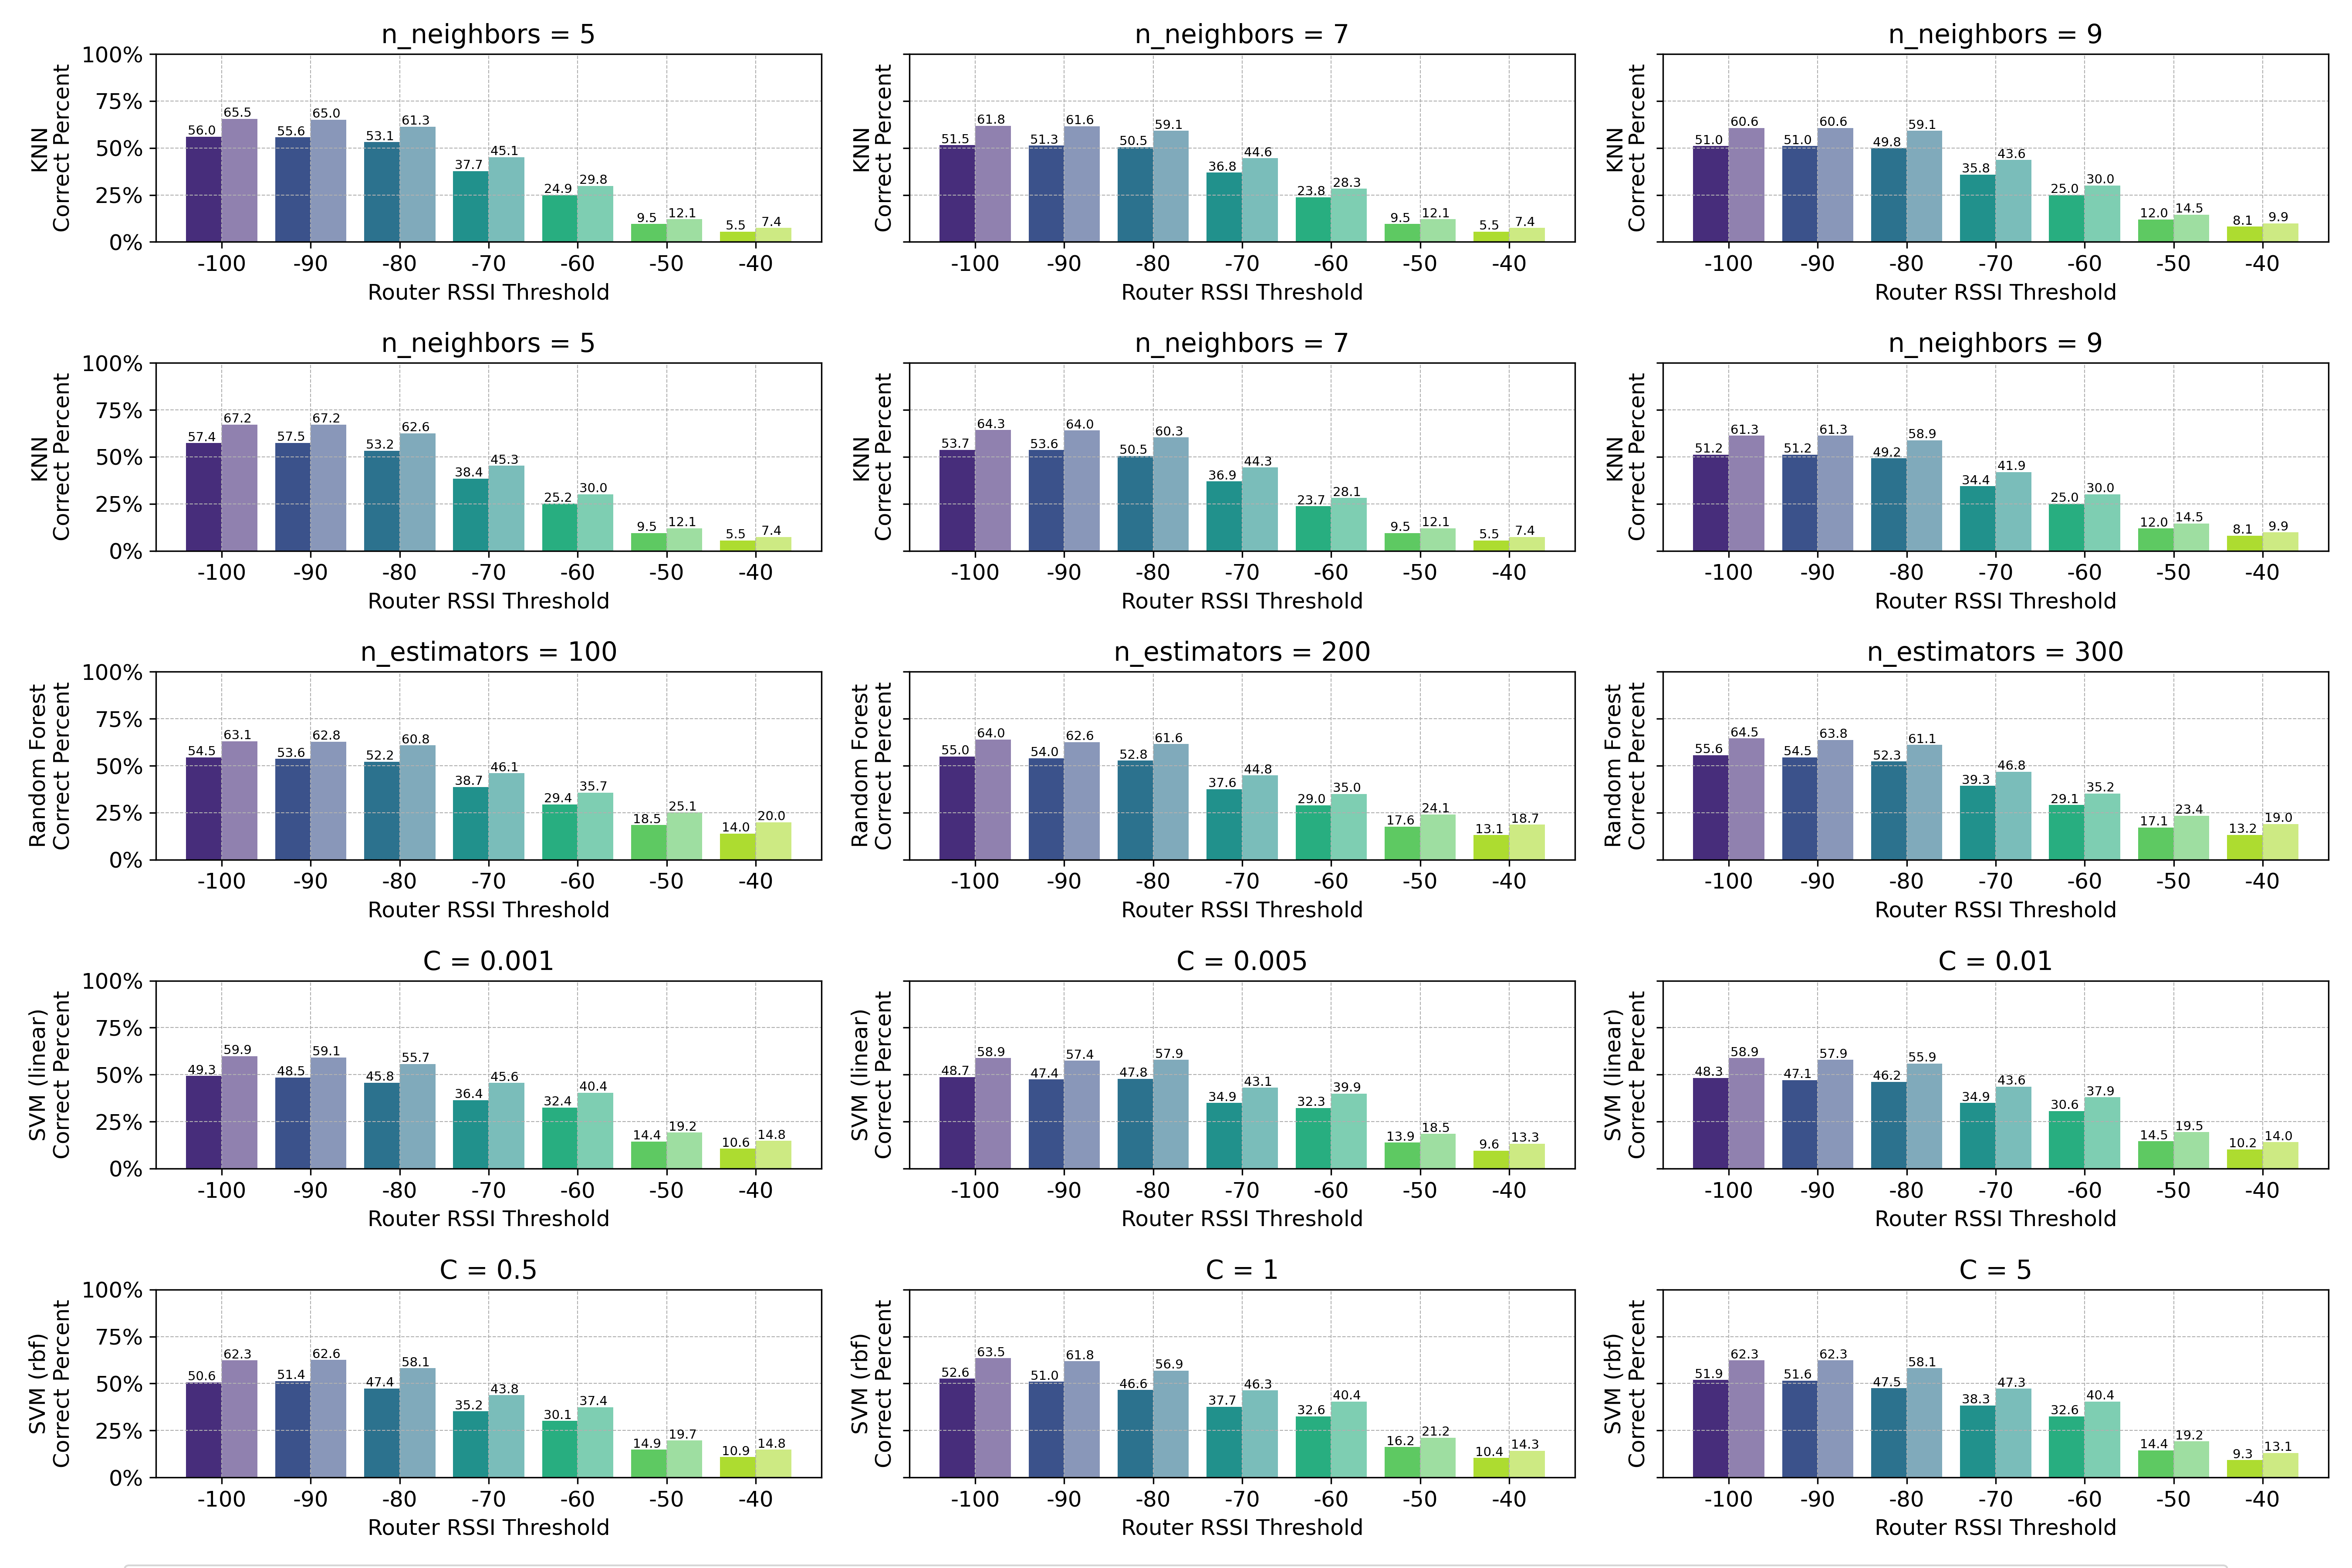
\includegraphics[width=0.8\textwidth]{images/6_router_rssi_threshold_01.png}
    \caption{Router Rssi Threshold}
    \label{fig:6_router_rssi_threshold_01}
\end{figure}

\subsection{Skalierung von RSSI-Werten}

\subsubsection{Formeln}

Quelle XX: Comprehensive analysis of distance and similarity measures for Wi-Fi fingerprinting indoor positioning systems

Die Idee hinter der Werteskalierung stammt aus der Quelle XX und basiert auf der Erkenntnis, dass die RSSI-Werte nicht linear verteilt sind. Durch eine geeignete Skalierung kann der Zusammenhang zwischen Entfernung und RSSI-Wert besser abgebildet werden. In der vorliegenden Arbeit wurden drei Skalierungsmethoden aus der Quelle XX implementiert und verglichen.

Grundlage jeder Skalierung ist die positive Darstellung der Werte. Hierfür wird von allen RSSI-Werten aus den Trainings- und Testdaten der niedrigste gemessene RSSI-Wert minus 1 subtrahiert:

\begin{equation}
    \text{Positiv}_i(x) = \text{RSS}_i - \text{min}
    \label{eq:positive_values_representation}
\end{equation}

wobei \(\text{min}\) der niedrigste RSS-Wert minus 1 ist, der alle Fingerabdrücke und WAPs in der Datenbank berücksichtigt.

Anschließend werden die Werte auf drei verschiedene Arten skaliert: linear, exponentiell und potenziert.

**Lineare Normalisierung:**

Die linear normalisierten Werte werden berechnet als:

\begin{equation}
    \text{NullBisEinsNormalisiert}_i(x) = \frac{\text{Positiv}_i(x)}{-\text{min}}
    \label{eq:linear_normalized_values}
\end{equation}

**Exponentielle Skalierung:**

Die exponentiell skalierten Werte werden berechnet unter Verwendung von \(\alpha = 24\):

\begin{equation}
    \text{Exponentiell}_i(x) = \frac{\exp\left(\frac{\text{Positiv}_i(x)}{\alpha}\right)}{\exp\left(\frac{-\text{min}}{\alpha}\right)}
    \label{eq:exponential_representation}
\end{equation}

**Potenzierte Skalierung:**

Die potenzierten Werte werden berechnet unter Verwendung von \(\beta = e\):

\begin{equation}
    \text{Potenz}_i(x) = \left(\frac{\text{Positiv}_i(x)}{-\text{min}}\right)^{\beta}
    \label{eq:powered_representation}
\end{equation}

In Abbildung \ref{fig:value_scaling_strategies_ignore_10} sind die verschiedenen Skalierungsmethoden dargestellt.

\begin{figure}[H]
    \centering
    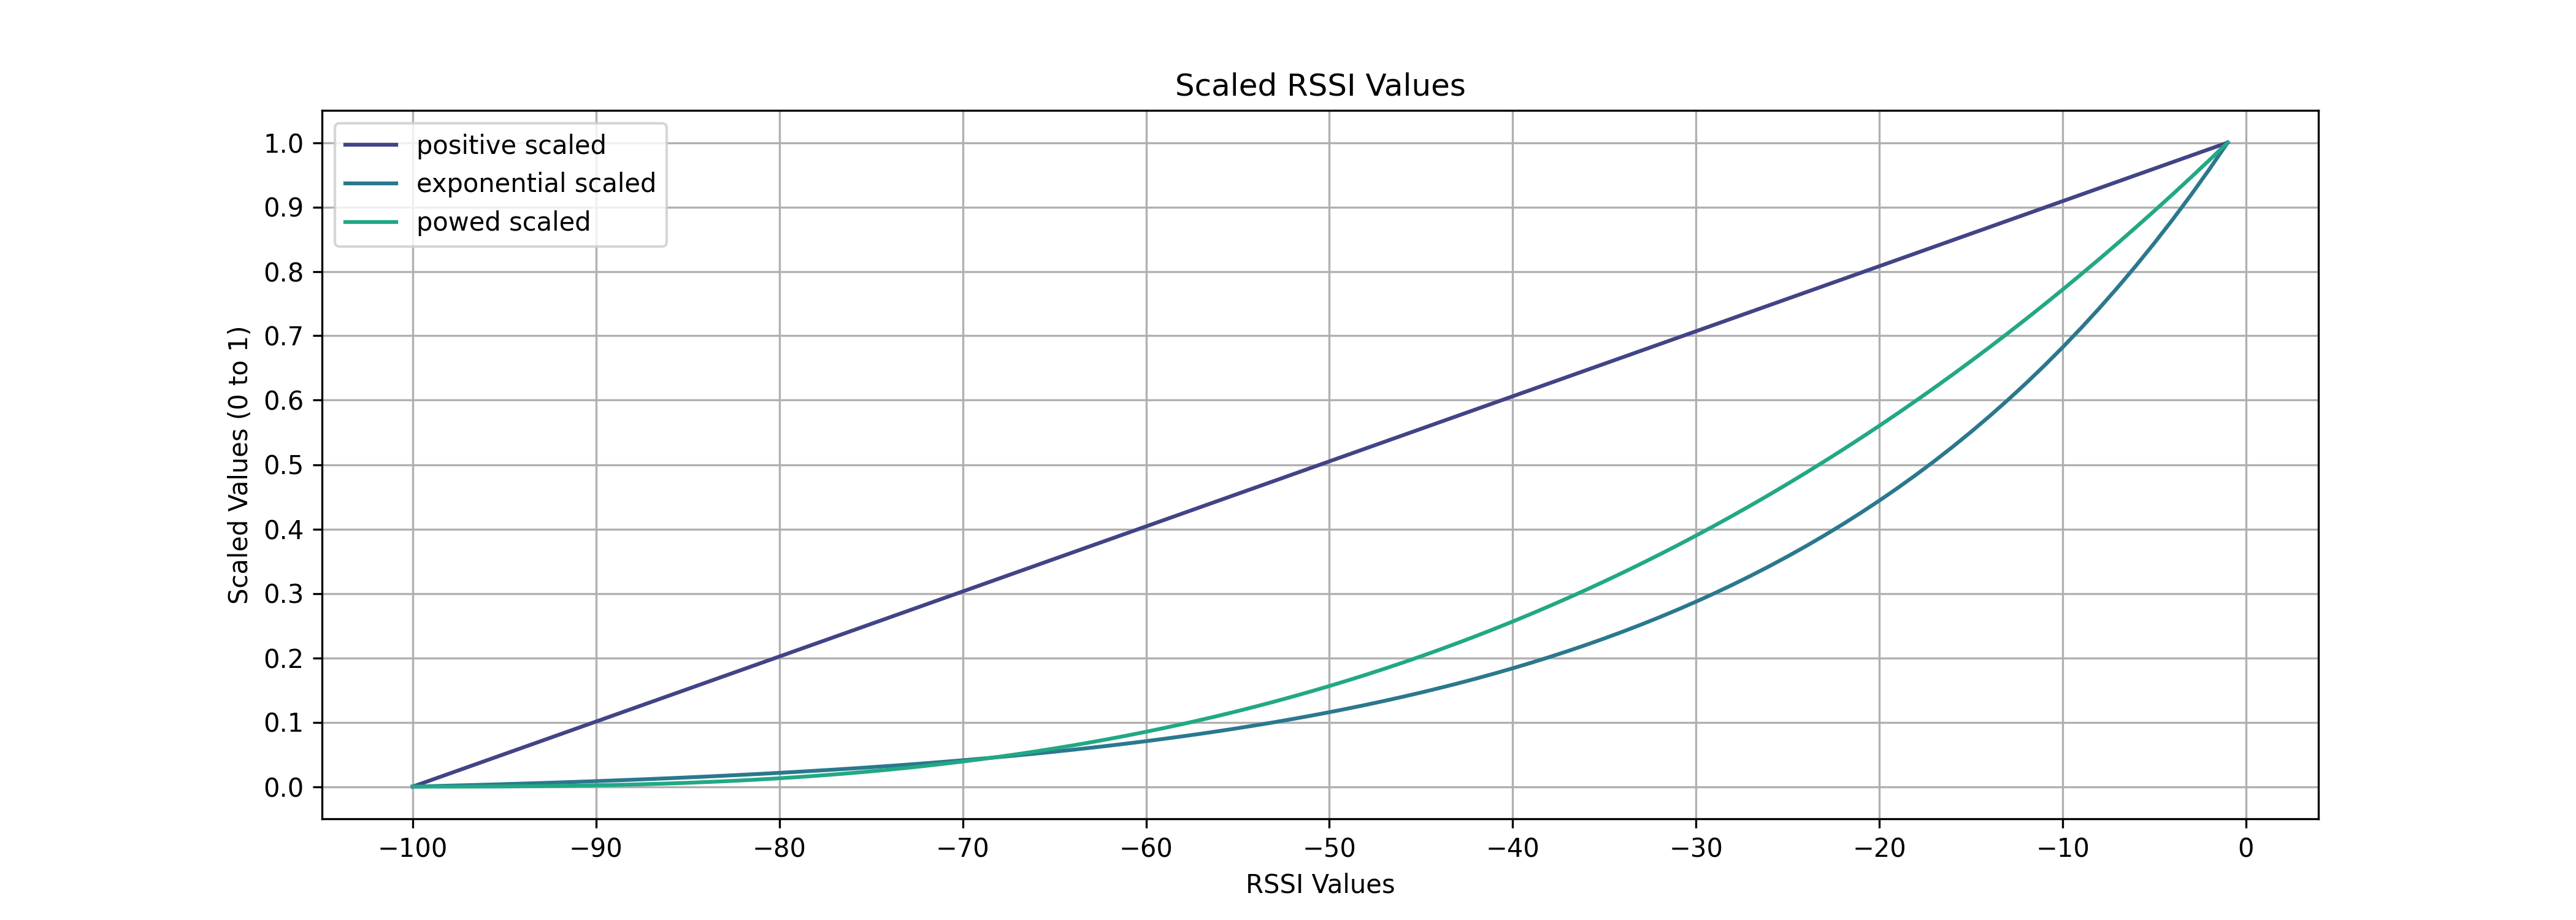
\includegraphics[width=0.8\textwidth]{images/value_scaling_strategies_ignore_10.png}
    \caption{Value Scaling Strategies}
    \label{fig:value_scaling_strategies_ignore_10}
\end{figure}


\subsubsection{Nochmal KNN Uniform vs. Distance}

Durch die Skalierung könnte es sein, dass die ursprüngliche Wahl der distance KNN Methode nicht mehr die beste ist. Aus diesem Grund wird vor der Untersuchung der Skalierungsmethoden nochmal der Vergleich zwischen distance und uniform durchgeführt in Zusammenhang mit den Skalierungsmethoden.

\begin{figure}[H]
    \centering
    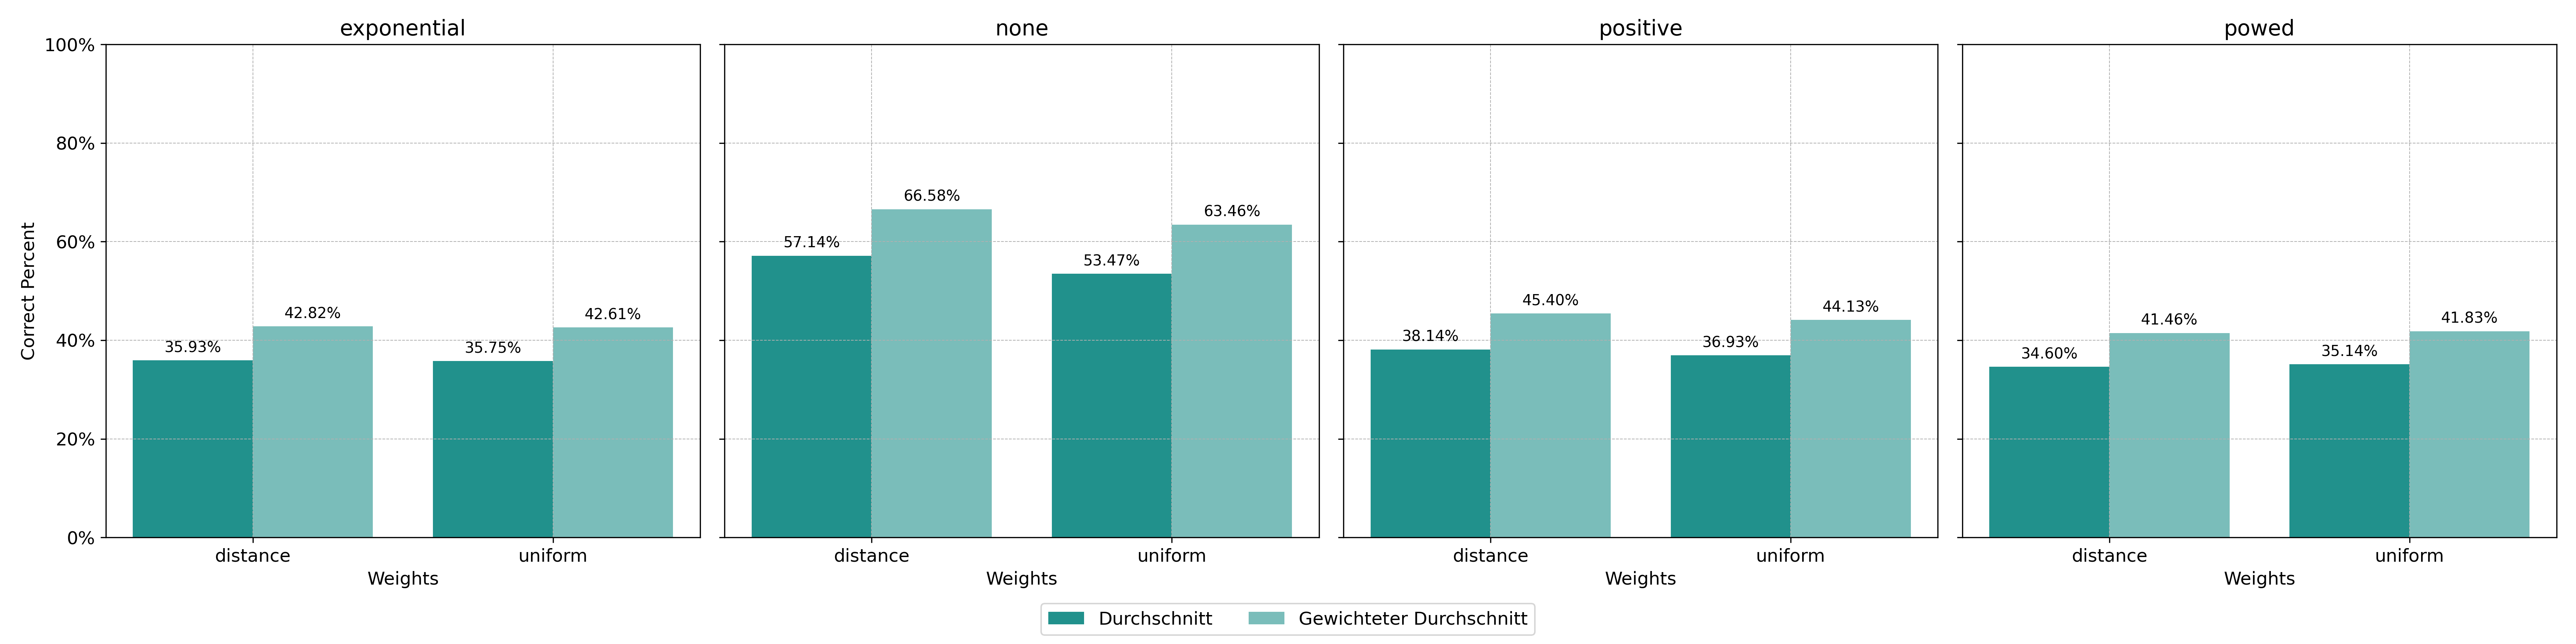
\includegraphics[width=0.8\textwidth]{images/7_value_scaling_strategy_knn_distance_02.png}
    \caption{KNN Uniform vs. Distance im Durchschnitt}
    \label{fig:7_value_scaling_strategy_knn_distance_02}
\end{figure}

\begin{figure}[H]
    \centering
    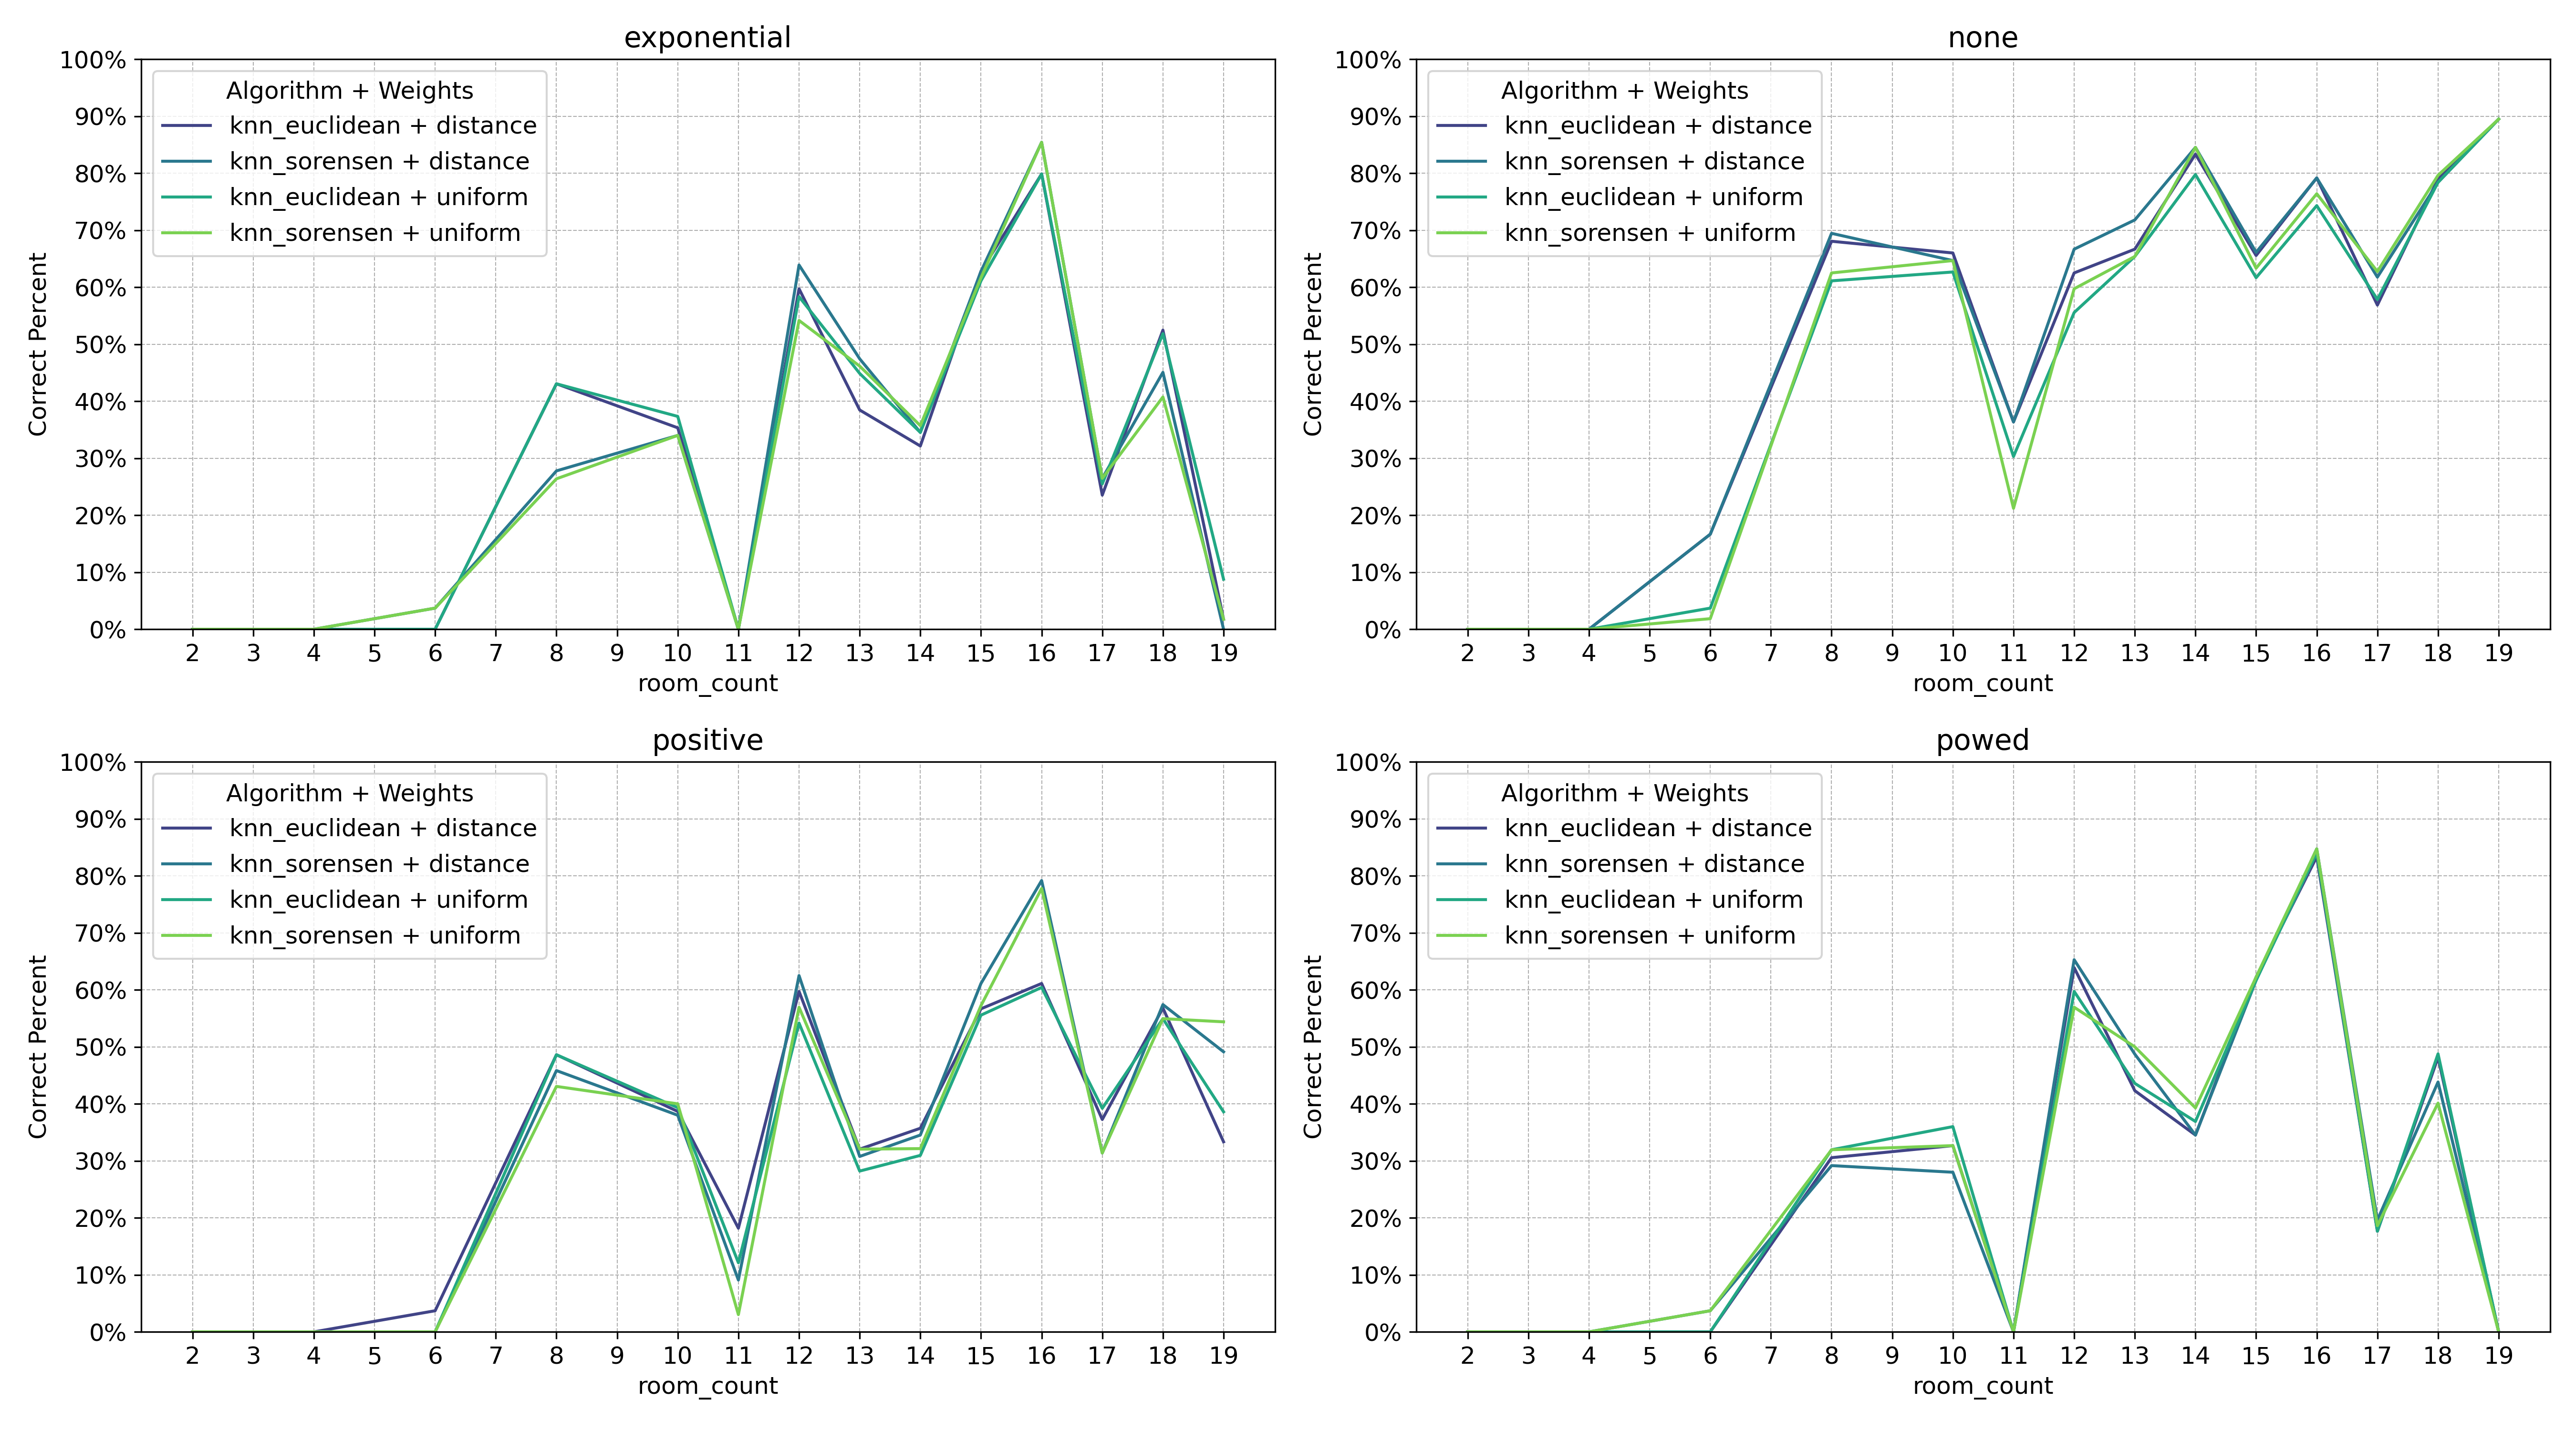
\includegraphics[width=0.8\textwidth]{images/7_value_scaling_strategy_knn_distance_03.png}
    \caption{KNN Uniform vs. Distance pro Raum}
    \label{fig:7_value_scaling_strategy_knn_distance_03}
\end{figure}

Wie zu erkenne ist, ist distance weiterhin besser als uniform. Aus diesem Grund wird weiterhin die distance weights Methode verwendet.

In Abbildung \ref{fig:7_value_scaling_strategy_02} folgendes zu erkennen:

\begin{itemize}
    \item In den meisten fällen sehr ähnlicher Verlauf --> Es gibt Unterschiede bei den Skalierungsmethoden, aber bei den Skalierungsmethoden sind die Ergebnisse bei euclidean/sorensen und distance/uniform sehr ähnlich
    \item Bei exponential: distance ist besser als uniform bei wenigen Messungen pro Raum
    \item Bei none: distanz ist etwas besser als uniform bei wenigeren Messungen. Abstand nimmt aber ab mit der Anzahl an Messungen
    \item Bei exponential, powed (und auch leicht bei positive): Nimmt die Genauigkeit mit zunehmender Anzahl an Messungen wieder ab. Bisher hatten die Räume mit den meisten Messungen immer die größten Genauigkeiten. In diesem Fall haben die Räume mit 16 Messungen die höchste Genauigkeit und danach nimmt es wieder ab. Bei exponential und powed ist die Genauzigkeit bei n = 19 sogar wieder bei fast allen Kombinationen aus distance und weights bei 0\%!
\end{itemize}

\begin{figure}[H]
    \centering
    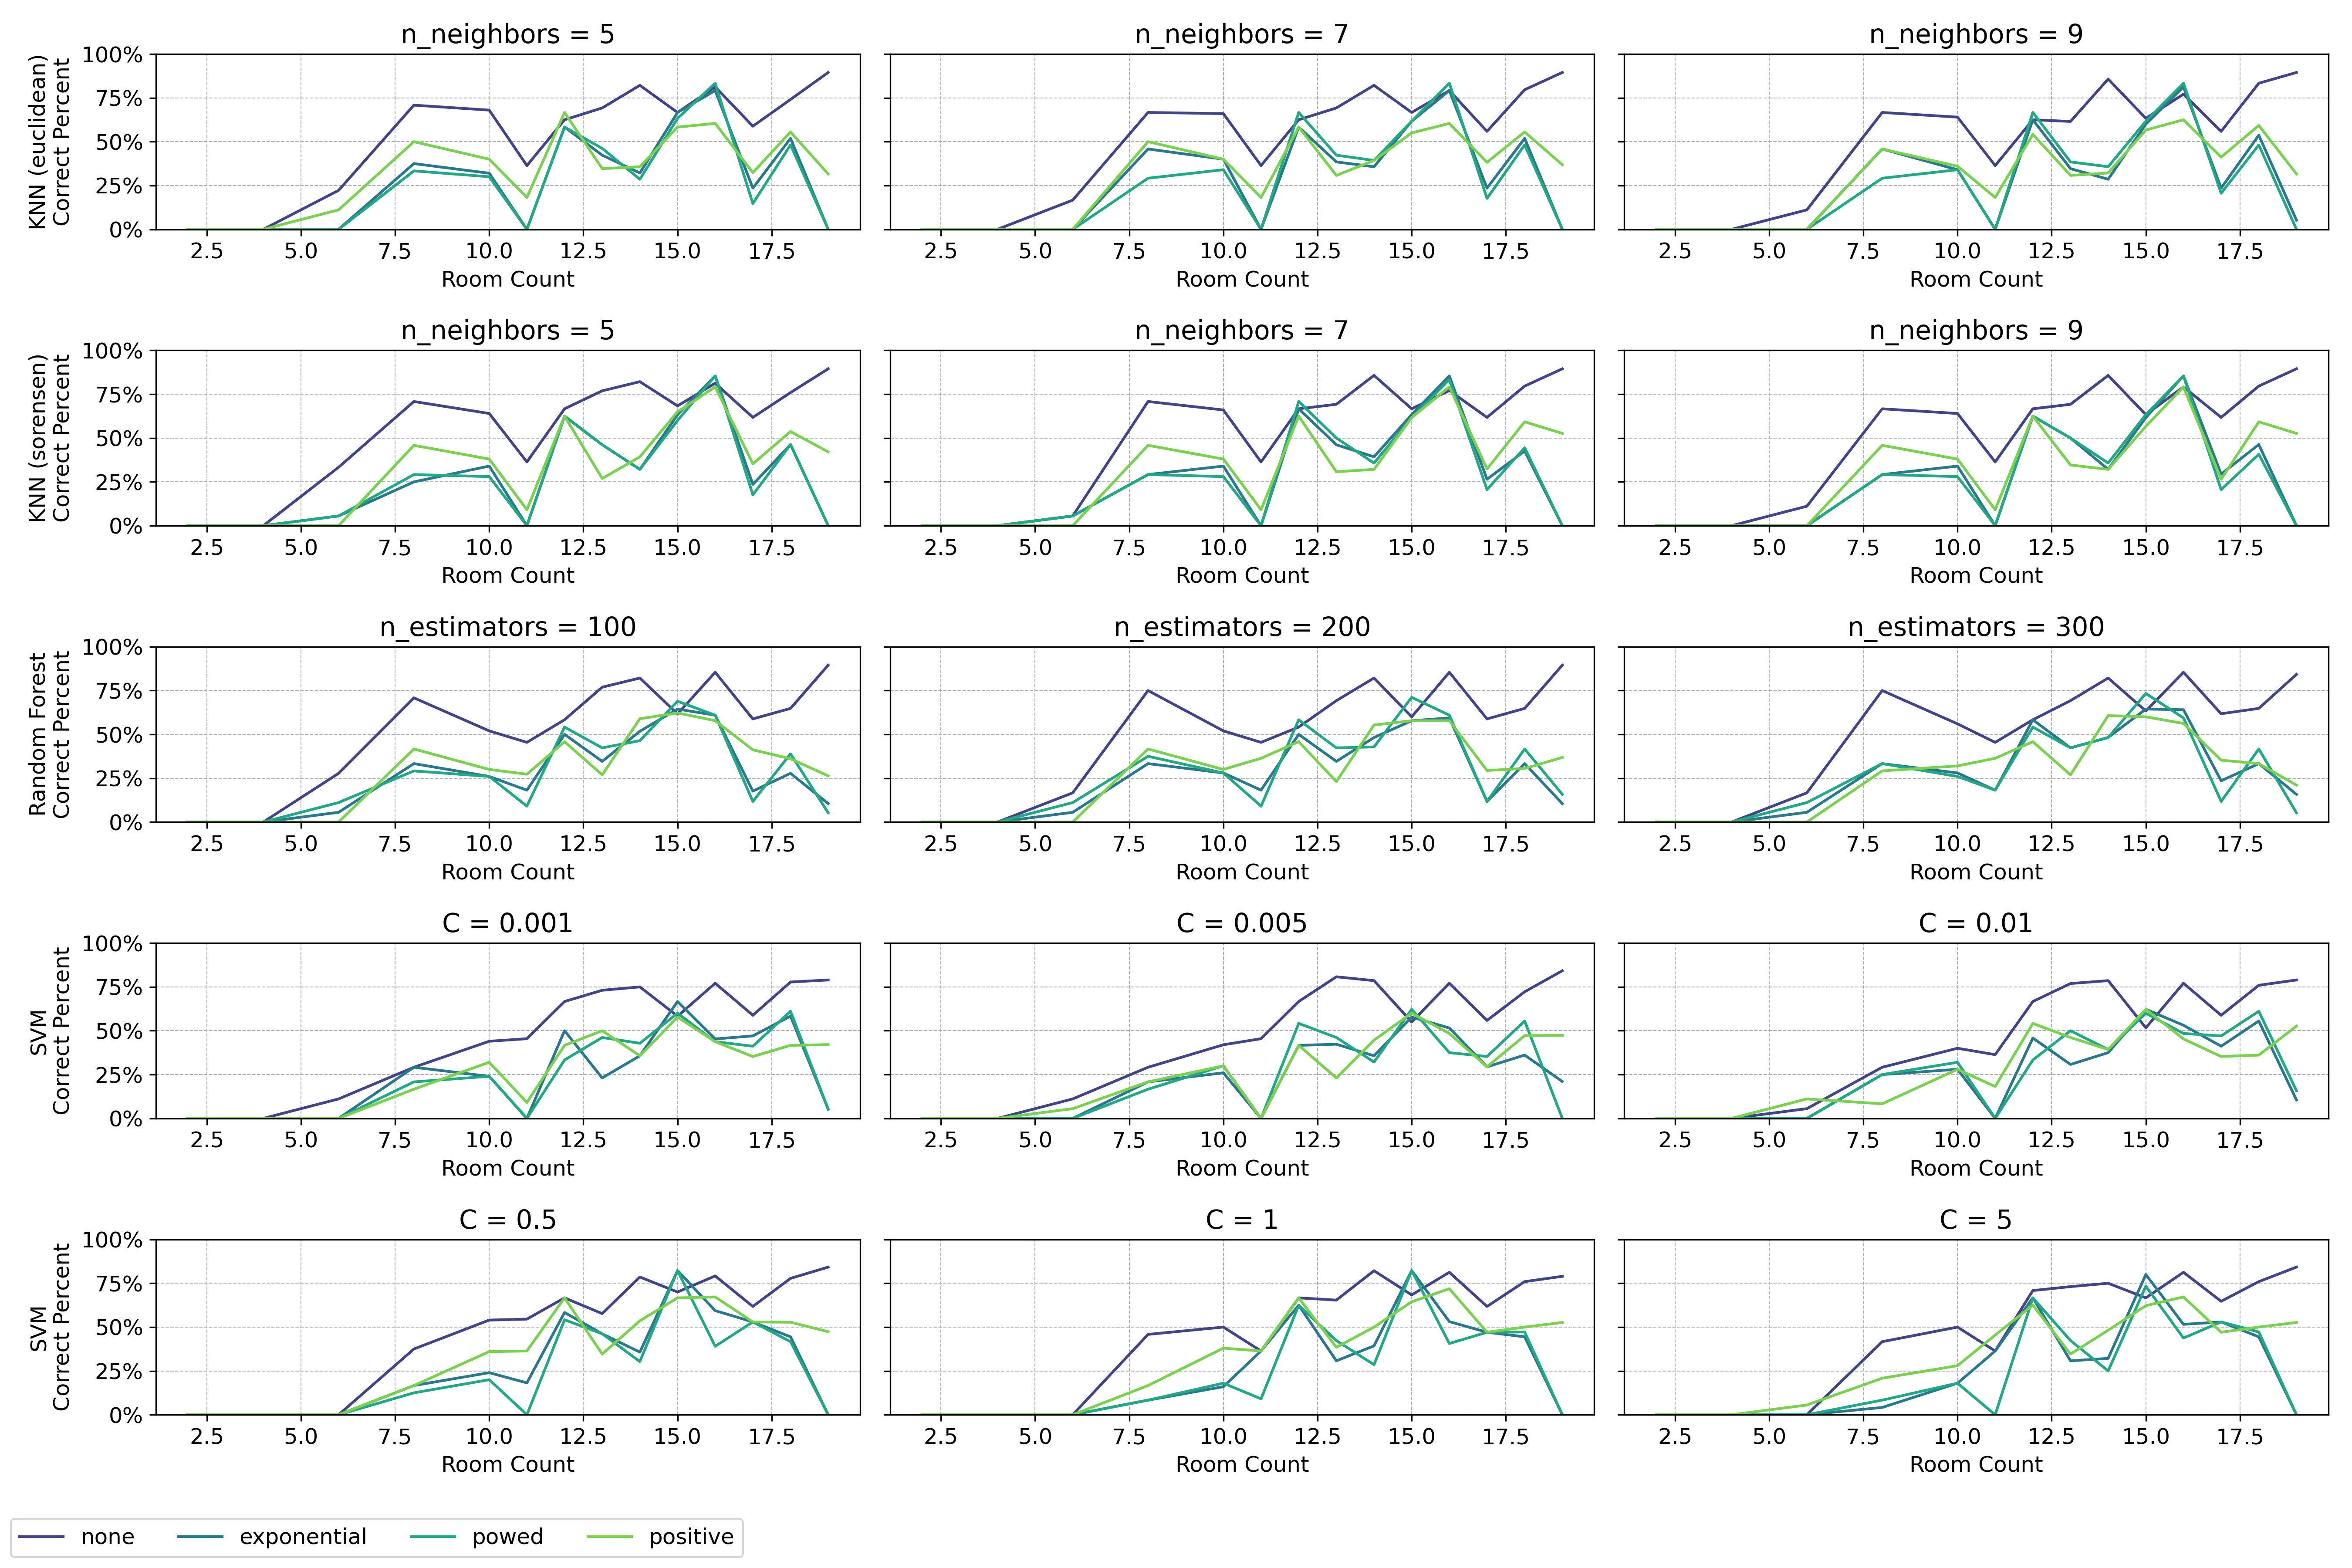
\includegraphics[width=0.8\textwidth]{images/7_value_scaling_strategy_02.png}
    \caption{Skalierungsstrategeien nach Algorithmus und Parameter pro Anzahl Messungen pro Raum}
    \label{fig:7_value_scaling_strategy_02}
\end{figure}

\section{Erweiterte Untersuchungen}

\subsection{Einfluss der Anzahl der Fingerprints auf die Genauigkeit}

In der folgenden Untersuchung wird im Detail untersucht, wie sich die Anzahl an Messungen auf die Genauigkeit der Ergebnisse wiederspiegelt. Dafür werden in diesem Fall die Trainingsdaten erweitern, sodass in 4 nahegelgenen Räumen je 20 Messungen gemacht wurden. Aufgrundlage dieser Messungen wird nun überprüft, wie sich der bis jetzt beste Algorithmus schlägt.

TODO: Lineplot mit den Ergebnissen (So wie die Heatmap, aber halt nur eine Achse)

\subsection{Verbesserung der Vorhersagegenauigkeit durch Fingerprints außerhalb der Räume}

Für eine noch bessere Genauigkeit wurde jetzt untersucht, wie sich die Genauigkeit verbessert, wenn zusätzlich zu den Fingerabdrücken innerhalb der Räume auch Fingerabdrücke außerhalb der Räume verwendet werden und somit auch vorhergesagt werden kann, dass kein korrekter Raum ermittelt werden konnte. Das ist sinnvoll, da in diesen Fällen die ESP32 keine Messdaten für falsche Räume veröffentlichen bzw. in weniger Fällen flasche Ergebnisse veröffentlichen kann.

\begin{figure}[H]
    \centering
    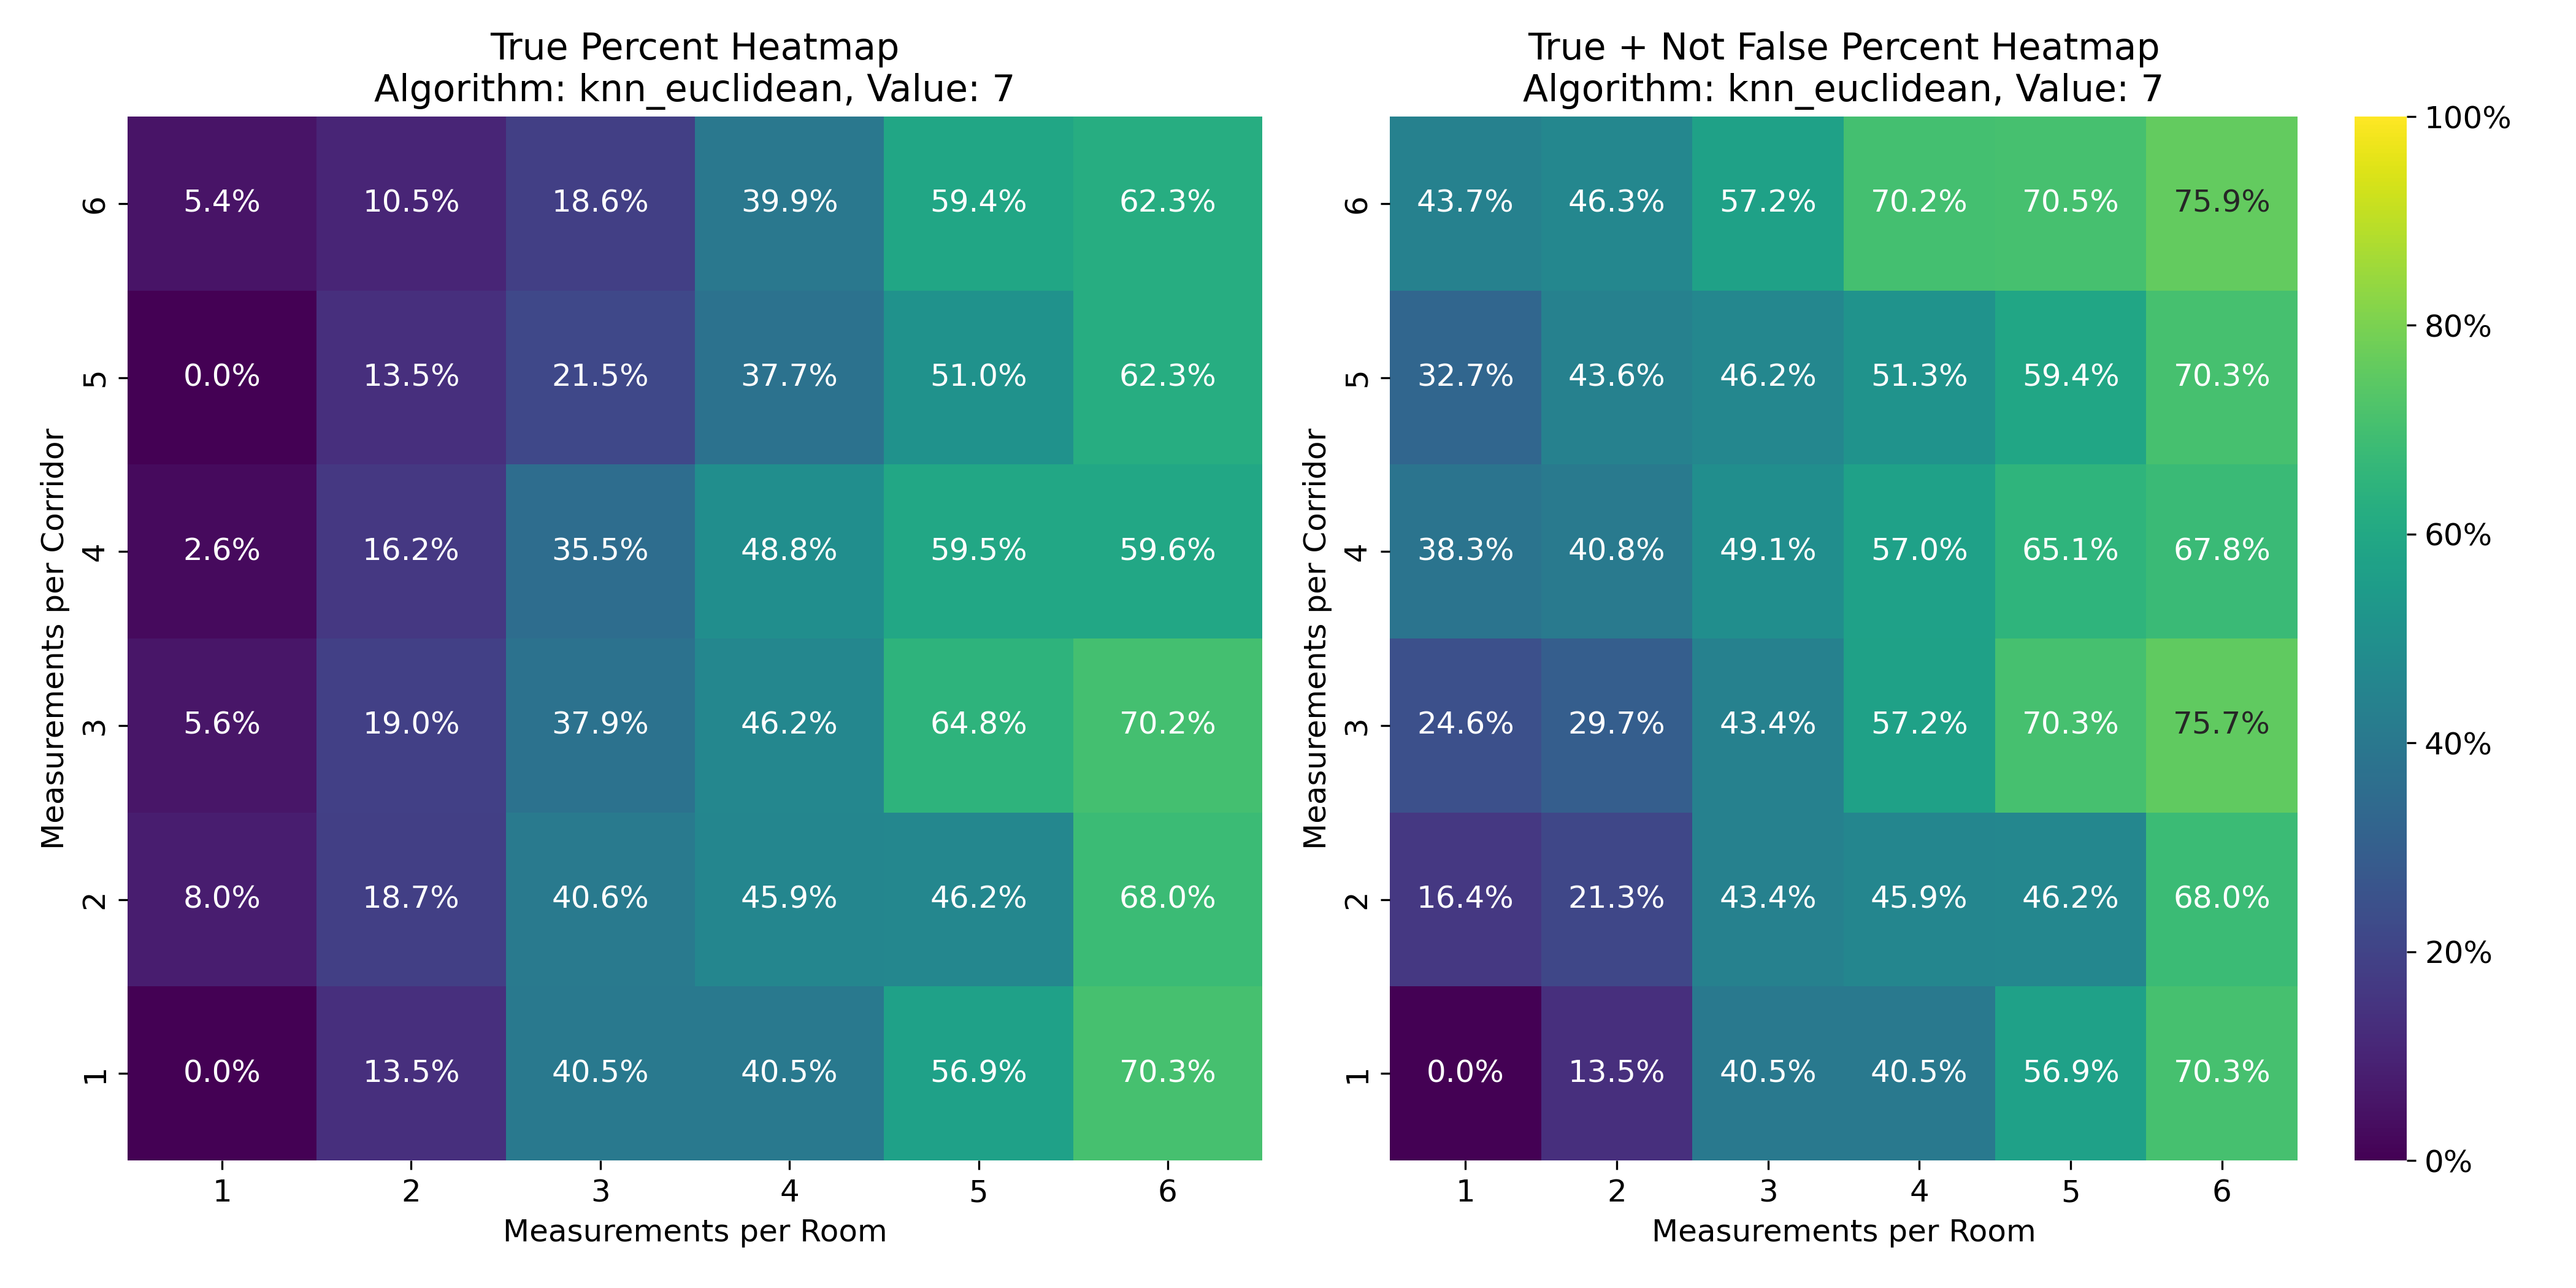
\includegraphics[width=0.8\textwidth]{images/8_test_corrdior_01.png}
    \caption{Ergebnisse unter Betrachtung von Messungen außerhalb der Räume}
    \label{fig:8_test_corrdior_01}
\end{figure}
